%%%%%%%%%%%%%%%%%%%%%%%%%%%%%%%%%%%%%%%%%%%%%%%%%%%%%%%%%%%%%%%%%%%%%%%%%%%%%%%%%%%%%%%%%%%%%%%%%%%%
% ==================================================================================================
% --------------------------------------------------------------------------------------------------
\chapter{Methodology}
In this section we motivate and introduce the proposed model, and explore its parametrization.
Wherever possible, concepts related to segmentation and classification will be described in their most general sense, since many of the these may also apply to other image analysis and machine learning tasks.
%%%%%%%%%%%%%%%%%%%%%%%%%%%%%%%%%%%%%%%%%%%%%%%%%%%%%%%%%%%%%%%%%%%%%%%%%%%%%%%%%%%%%%%%%%%%%%%%%%%%
\section{Model Design}\label{s:modelconcept}
As suggested in \S\ \ref{ss:priorproposed}, three general paradigms have emerged for segmentation of brain MRI.
The first and most popular is the pipeline, in which sub-tasks are completed in sequence, such as: pre-processing, classification, post-processing.
This approach permits a flexible model definition which can incorporate existing algorithms for individual steps.
Most thresholding and classic supervised models fall under this category.
The main drawback of this approach is that some steps could be improved by the results of downstream steps.
For example, tissue classifying modules typically assume that the bias field is already corrected, but bias field estimation can be more accurate if the tissue segmentation is known.
\par
The second paradigm, a unified generative model, aims to solve this chicken-egg problem.
The segmentation is parameterized in one integrated probabilistic model, which often combines the input images with tissue prior probability images, a bias field model, and smoothness terms.
Parameters of each sub-model are estimated using several expectation maximization (EM) iterations before the final segmentation is inferred.
The challenges to this approach include balancing model complexity with estimability, robust convergence issues, and reduced ability to include external tools.
\par
The final paradigm, deep learning, uses error back-propagation to update thousands of parameters in a large, relatively unstructured model mapping the input MRI to the output segmentation image.
Using so-called ``end-to-end'' training, there is no guarantee that the usual sub-components (e.g. bias field, tissue graylevel distributions, etc.) will be estimated, though such elements could be expected to develop in the internal relationships if they are relevant to the task at hand.
Most deep learning models still require standardization in space and graylevel, and more importantly, large training datasets -- which are rare in medical imaging.
\par
For several reasons, the supervised pipeline approach was selected for this work.
First, preliminary work drawing on existing algorithms \cite{Khademi2014,Schmidt2015} showed the feasibility of several relatively simple thresholding methods, which confer robustness through simplicity.
Second, the parametric assumptions required by unified probabilistic models may be challenged by data from multiple sources \cite{VanLeemput2001}.
Third, only a small number of training cases were available during initial development, which limited the feasibility of deep learning approaches.
Finally, time constraints favoured the incorporation of existing tools to address challenges like bias correction and image registration, which would have been otherwise difficult to develop in a unified model.
% ==================================================================================================
\subsection{Features}
Many FLAIR-only WMH segmentation algorithms use a thresholding technique: map a single graylevel feature directly to a class or class probability (e.g. ``healthy'' or ``lesion'').
Such models often have complex methods of deriving this mapping (e.g. using mixture model parameters \cite{Roura2015}, histogram features \cite{Yoo2014}, or conditional edge probability \cite{Knight2016}), but the final rule is applied equally to the entire graylevel image, usually the FLAIR sequence.
The most common challenge for these methods is a high number of false positives (cf. \S\ \ref{ss:metrics} for definitions), since several artifacts and GM can overlap the WMH intensity distribution.
As a result, nearly all previously proposed thresholding algorithms employ heuristic ``false positive reduction'' (FPR) rules as post-processing to remove these errors.
\par
% Need to introduce registration \& MNI space earlier (\cite{Evans1993})
Preliminary investigations sought to characterize the spatial distribution of false positives, in order to explore possible FPR rules.
Using a database of 96 FLAIR images in MNI space (cf. \S\ \ref{ss:data} for details), the optimal threshold for each image was calculated%
\footnote{The \texttt{fminsearch} function in Matlab maximized the similarity index with respect to the manual segmentation.}
and used to generate binary class images ($0 =$ healthy, $1 =$ lesion).
Comparing these results with the manual segmentations, the average distribution of true positives (TP), false positives (FP), and false negatives (FN) was computed, as shown in Figure \ref{fig:thropt-tpfpfn}.
The median optimal similarity index (SI) was 0.36.
\begin{figure}[h]
  \centering
  \begin{subfigureside}{TP}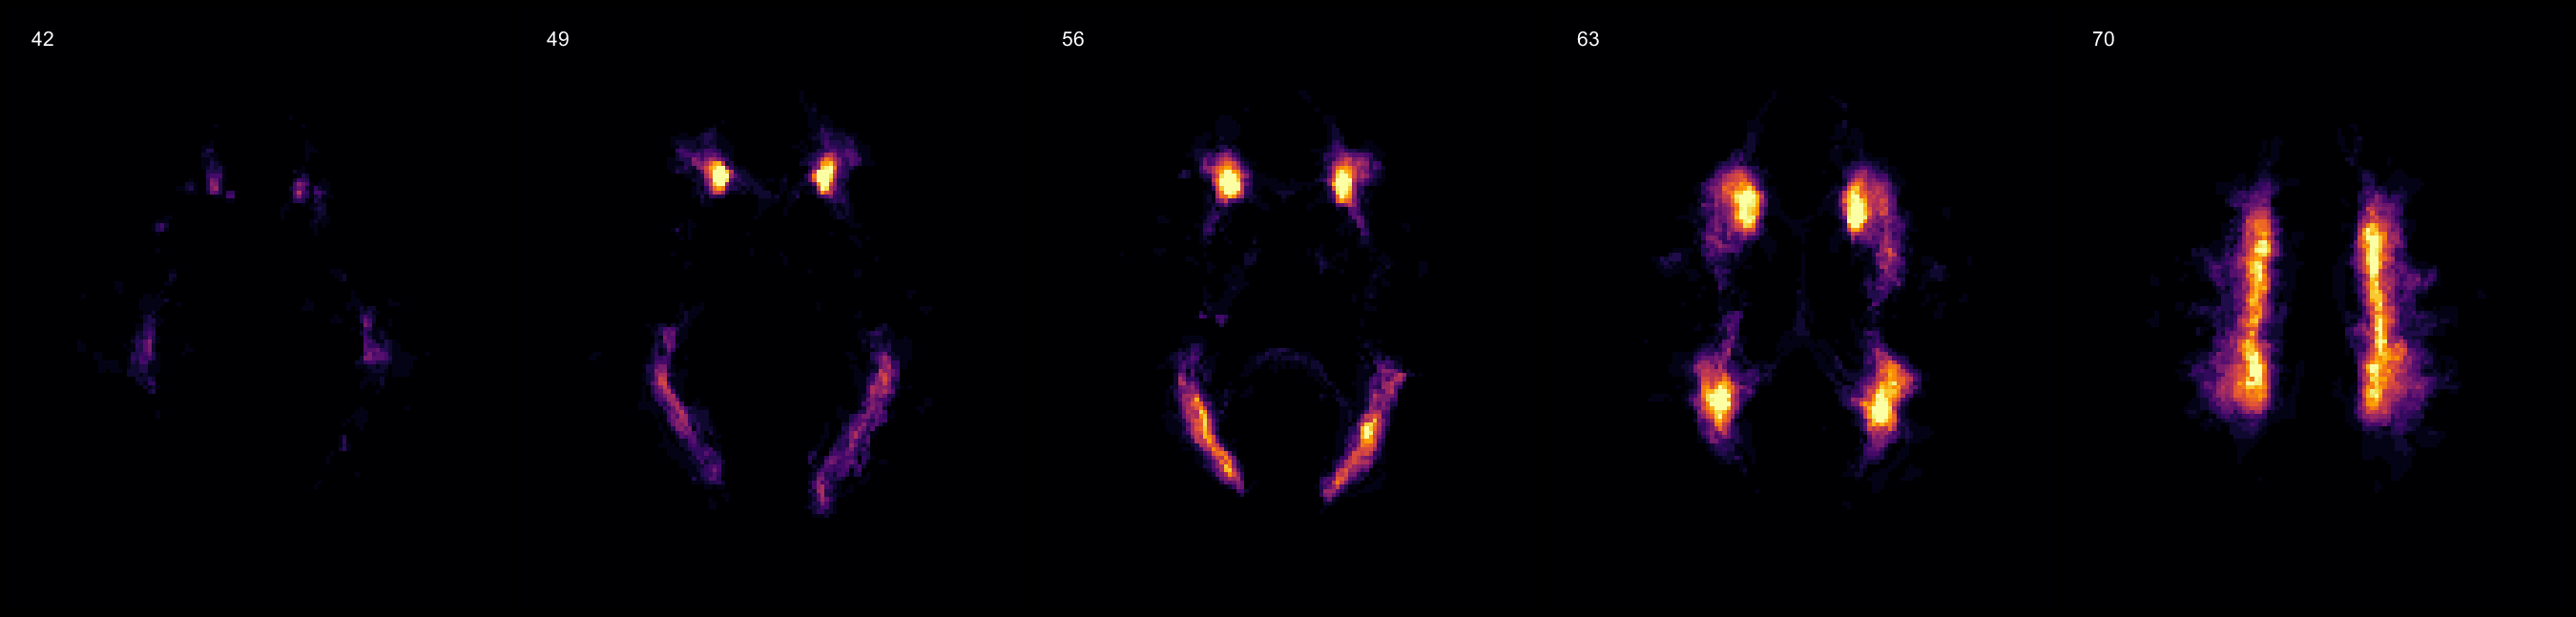
\includegraphics[height=\sliceheight]{rawthropt-tp.png} 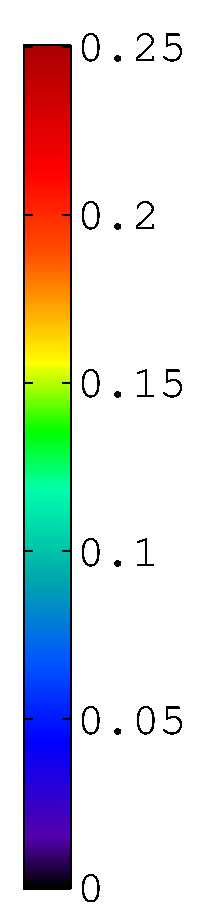
\includegraphics[height=\sliceheight]{cbar-NIH3-0-025}\end{subfigureside}\\[0.5em]
  \begin{subfigureside}{FP}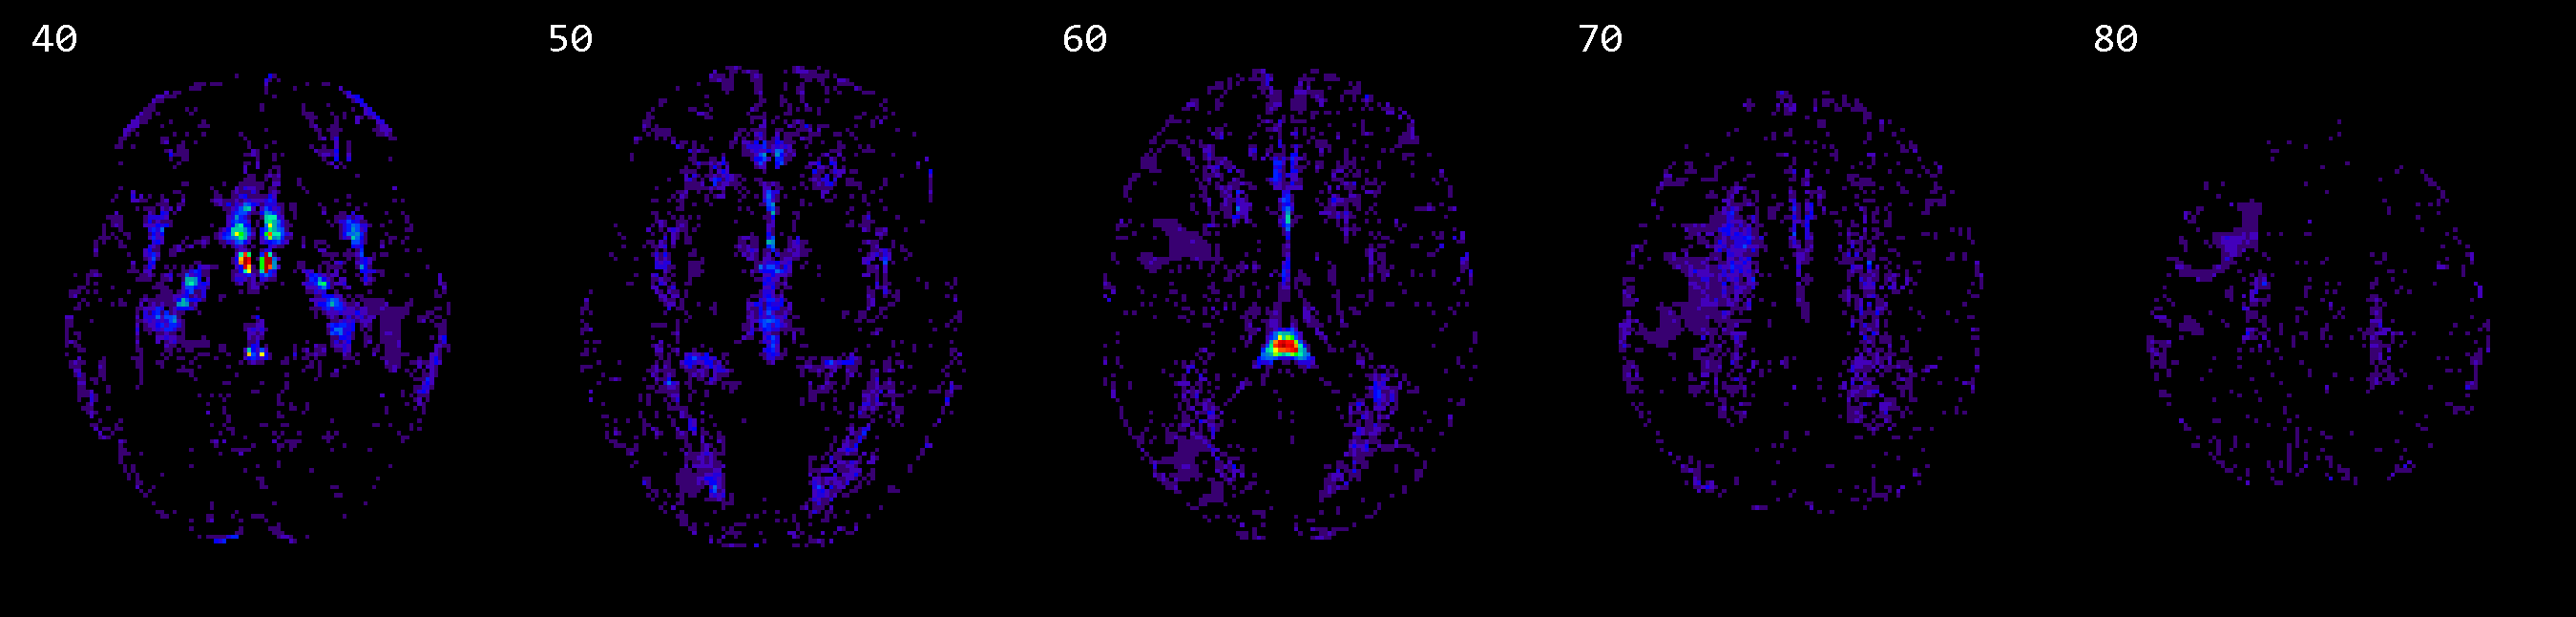
\includegraphics[height=\sliceheight]{rawthropt-fp.png} 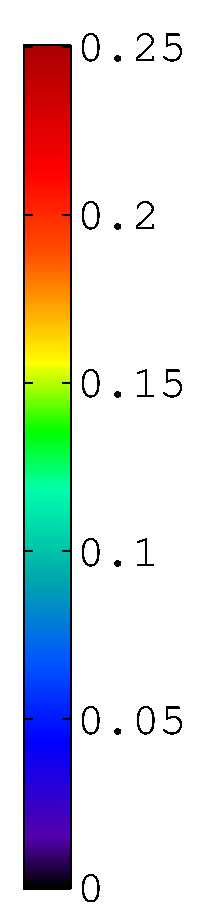
\includegraphics[height=\sliceheight]{cbar-NIH3-0-025}\end{subfigureside}\\[0.5em]
  \begin{subfigureside}{FN}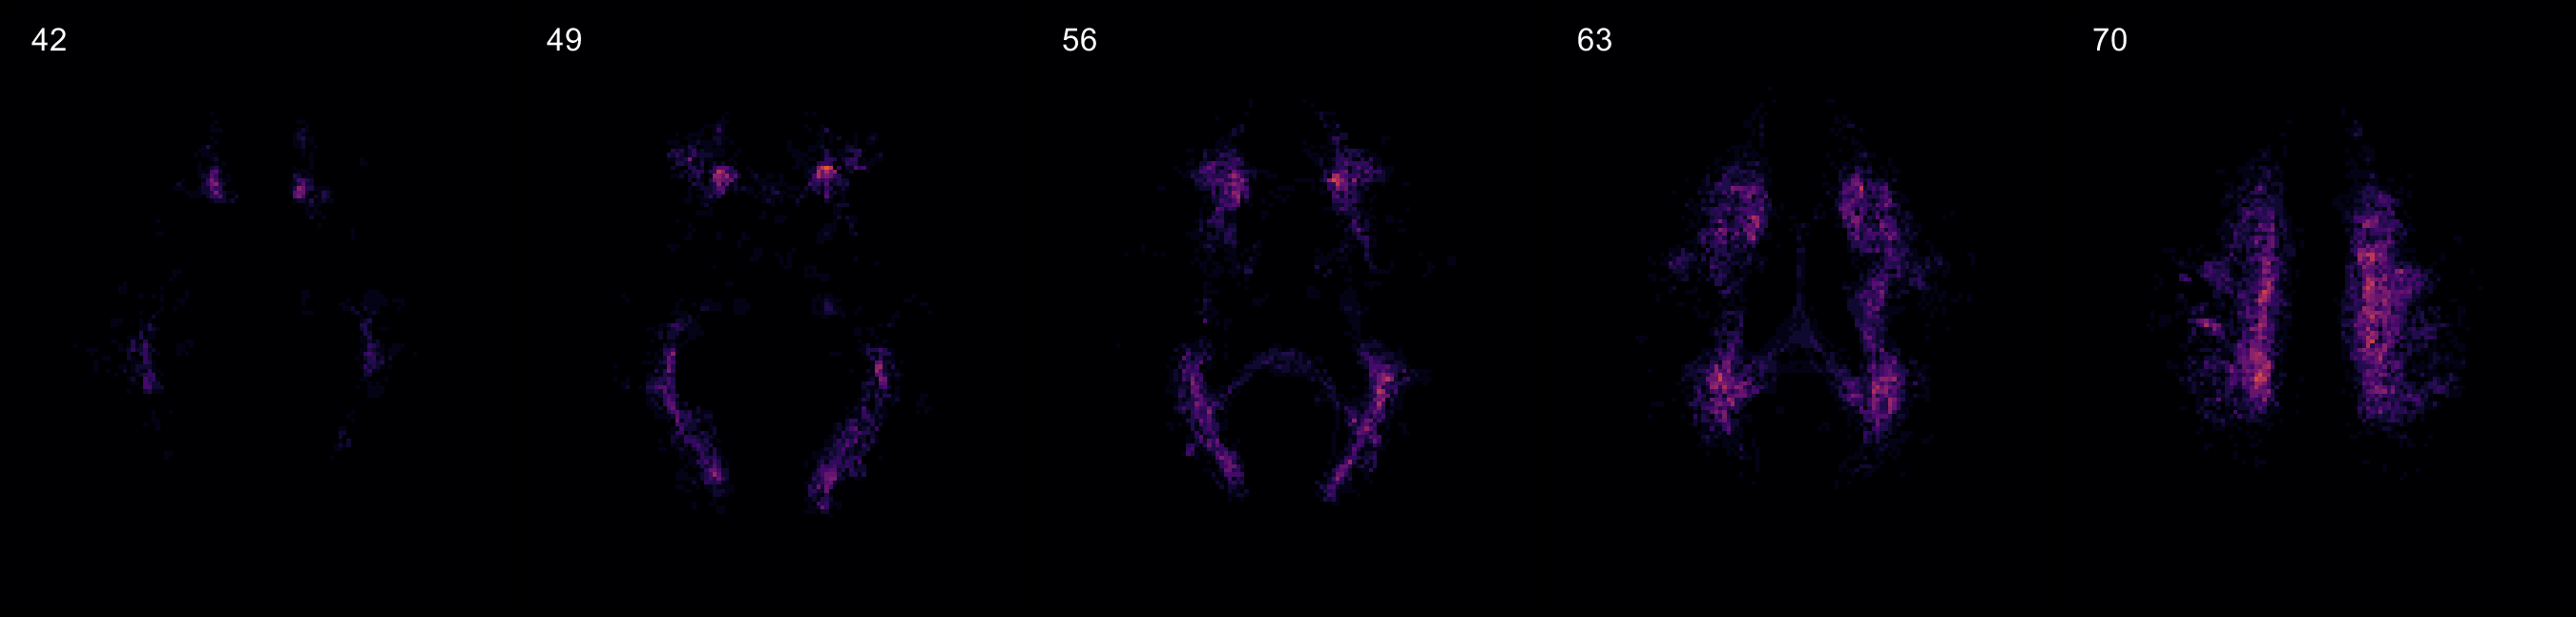
\includegraphics[height=\sliceheight]{rawthropt-fn.png} 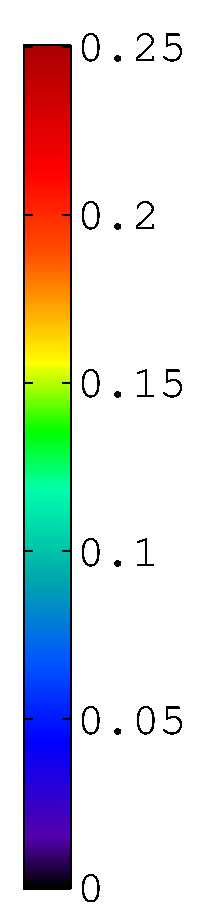
\includegraphics[height=\sliceheight]{cbar-NIH3-0-025}\end{subfigureside}s
  \caption{Distributions of TP, FP, and FN in 96 FLAIR MRI, following supervised optimal thresholding in MNI space.}
  \label{fig:thropt-tpfpfn}
\end{figure}
\par
Evidently, even if an optimal threshold could be estimated for these data, a high proportion of FP and FN would be incurred.
Yet in Figure \ref{fig:thropt-tpfpfn} there are regular and distinct spatial distributions of these errors.
Moreover, is it has been suggested that there is regional heterogeneity in relaxation rates of brain tissues \cite{Sled2004}, and that WML intensity depends in part on location \cite{Stevenson2000,Harmouche2015}.
This implies that spatial coordinates would be useful features for WMH segmentation, especially when incorporated into the main classification model (i.e. not as post-processing).
Indeed such features have previously been used \cite{Anbeek2004,Anbeek2005,Dyrby2008,Griffanti2016,Dadar2017}.
\par
Spatial features could be used with FLAIR intensities in supervised classification models like K-NN, SVM, RF, etc.
However, such models treat all features equally, which can lead to artifacts in the decision boundary that contradict prior knowledge.
For example, in spatial locations which do not observe any lesions during training, the optimized model may learn to never predict the lesion class, regardless of graylevel features.
Similarly, there is no guarantee that FLAIR graylevels will map monotonically to the lesion class, as would be expected.
Therefore, spatial features should be treated differently.
% ==================================================================================================
\subsection{Overview}
The proposed pipeline can be summarized as follows.
Pre-processing steps will aim to correct any bias field effect and standardize spatial coordinates.
The classification model will employ FLAIR intensities and spatial features to give the initial segmentation.
Since most classification models assume features are drawn from a consistent distribution, a graylevel standardization step is appended to the pre-processing.
Post-processing steps will generally aim to improve segmentation performance.
This pipeline is illustrated in Figure \ref{fig:pipeline}.
Next, the proposed classification model is developed.
\begin{figure}
  \centering\scalebox{0.65}{\pgfdeclarelayer{background}
\pgfdeclarelayer{foreground}
\pgfsetlayers{background,main,foreground}
\tikzset{%
  arrow/.style = { ->, >=Latex,  very thick, rounded corners, draw = #1!60!white },
  tbox/.style  = { fill = white, draw = #1!60!white, very thick, align = center }
}
\newcommand*{\textbox}[6]{%
  \node[tbox=#5,minimum width=#3cm,minimum height=#4cm]at(#1,#2){#6};
}

\newcommand*{\ix}{0.8}\newcommand*{\ixx}{1.6}
\newcommand*{\iy}{1}  \newcommand*{\iyy}{2}
\newcommand*{\pw}{1.5}
\newcommand*{\fw}{0.3}

% --------------------------------------------------------------------------------------------------
\begin{tikzpicture}
    \useasboundingbox(0.0, 0.0) rectangle (24.0,  2.0);
    \draw[black!30!white,rounded corners,very thick](00.0, 00.0) rectangle (24.0,  2.0);
    \textbox{ 2.0}{ 1.0}{3}{1}{black} {FLAIR MRI}
    \textbox{ 6.0}{ 1.0}{3}{1}{blue}  {Bias Correction\\\& Registration}
    \textbox{10.0}{ 1.0}{3}{1}{violet}{Graylevel\\Standardization}
    \textbox{14.0}{ 1.0}{3}{1}{red}   {Lesion\\Classification}
    \textbox{18.0}{ 1.0}{3}{1}{orange}{Post-Processing}
    \textbox{22.0}{ 1.0}{3}{1}{black} {Label Image}
    \draw[arrow={black}  ]( 3.5, 1.0)--( 4.5, 1.0);
    \draw[arrow={black}  ]( 7.5, 1.0)--( 8.5, 1.0);
    \draw[arrow={black}  ](11.5, 1.0)--(12.5, 1.0);
    \draw[arrow={black}  ](15.5, 1.0)--(16.5, 1.0);
    \draw[arrow={black}  ](19.5, 1.0)--(20.5, 1.0);
%    \draw[arrow={black} ]( 3.5, 1.0)--( 4.5, 1.0);
%    \draw[arrow={blue}  ]( 7.5, 1.0)--( 8.5, 1.0);
%    \draw[arrow={violet}](11.5, 1.0)--(12.5, 1.0);
%    \draw[arrow={red}   ](15.5, 1.0)--(16.5, 1.0);
%    \draw[arrow={orange}](19.5, 1.0)--(20.5, 1.0);
\end{tikzpicture}}
  \caption{Overview of the necessary processing steps.}
  \label{fig:pipeline}
\end{figure}
% address challenges here?
%- overlapping distributions \& hyperintense artifacts: spatial parametrization
%- bias field: correct beforehand
%- DAWM \& PVA: maintain probabilistic output 
%- image variability: graylevel standardization, image registration, spatial parametrization
%However, it has been suggested that there is regional heterogeneity in relaxation rates of brain tissues \cite{Sled2004}, and that WMH intensity depends in part on location \cite{Stevenson2000}.
%Many of the previously proposed WMH segmentation algorithms predict the class of a voxel without any spatial information.
%In the absence of spatial information, 
%The work by \citeauthor{Khademi2012} \cite{Khademi2012,Khademi2014,Khademi2015} was particularly promising, since it overcame many of the usual requirements.
%These include: the use of multiple MRI modalities, which are not always available; image registration to a common space, which is never perfect and introduces interpolation artifact; the use of training data, which is difficult to find; and assumed Gaussian distribution of tissue graylevels, which is rarely valid.
%Assumptions which many models make, and whether they are wrong:
%%- parametric modelling of graylevel distributions: with single Gaussians: almost certainly wrong.
%Confounding factors: PVA, parallel MRI signals, motion artifacts, 
%%The most recent implementation of the EM-fit mixture model by \citeauthor{Ashburner2005} in \cite{Ashburner2005} permits a user-specified number of Gaussian distributions for each tissue class, 
%However, 
%\begin{figure}
%  \centering
%  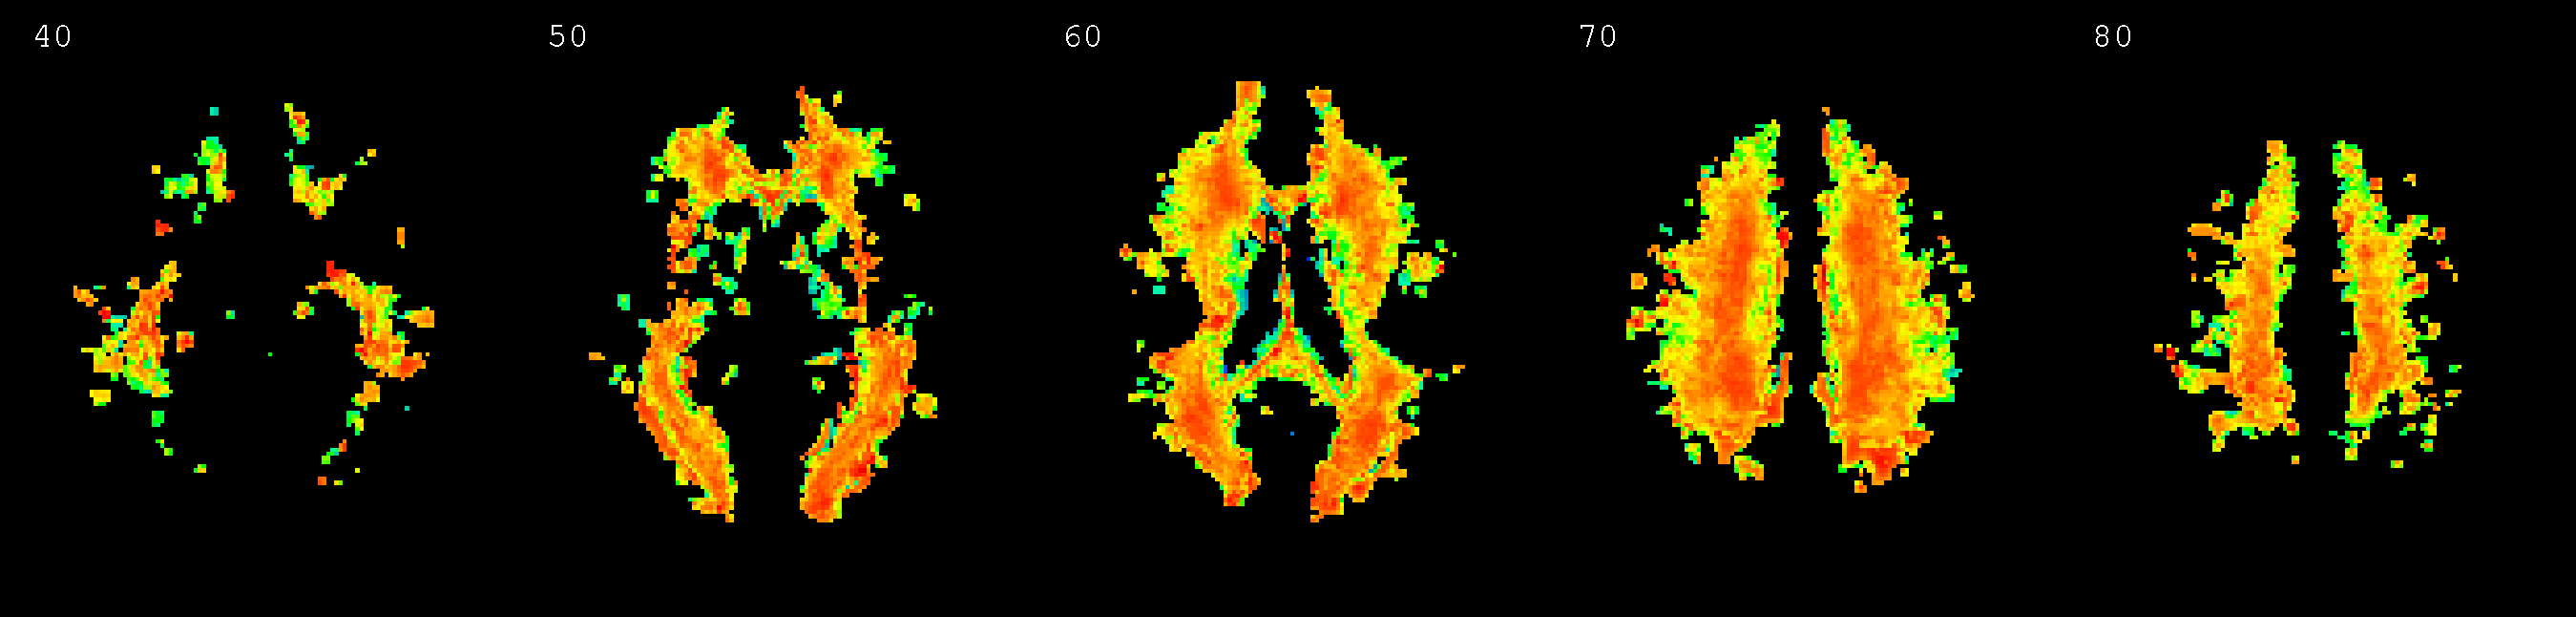
\includegraphics[height=\sliceheight]{meangray-c1.png}
%  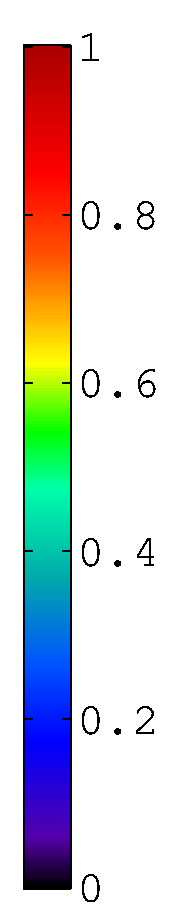
\includegraphics[height=\sliceheight]{cbar-NIH3-0-1.eps}
%  \caption{Mean lesion class graylevel after standardization in 96 coregistered FLAIR MRI.}
%  \label{fig:meangray-c1}
%\end{figure}
%%%%%%%%%%%%%%%%%%%%%%%%%%%%%%%%%%%%%%%%%%%%%%%%%%%%%%%%%%%%%%%%%%%%%%%%%%%%%%%%%%%%%%%%%%%%%%%%%%%%
\section{Voxel-Wise Logistic Regression}\label{s:vlr}
This section presents the proposed classification model: Voxel-wise Logistic Regression (VLR).
The VLR model solves the problem of differential treatment for spatial and graylevel features, and produces uniquely interpretable parameters following training.
The model is inspired by the LPA algorithm in the LST toolbox for SPM by \citeauthor{Schmidt2015} \cite{Schmidt2015,Schmidt2017a}%
\footnote{This algorithm was originally understood through the Matlab code, after downloading the toolbox. Section 6.1 of \cite{Schmidt2017a}, published in \citeyear{Schmidt2017a}, provides more details.}%
, however, novel methods of model parametrization and estimation are presented here, in addition to differences in pre- and post-processing from the LPA algorithm.
\par
Logistic regression models have recently gained popularity for WMH segmentation \cite{Sweeney2013a,Sweeney2013,Schmidt2017a,Zhan2017}, and have several advantages.
First, model parameters are generally more interpretable than those in other models, permitting better design of regularizations.
Second, the simplicity of the model reduces its capacity for over-fitting.
Third, model foundations in statistical theory allow probabilistic interpretations of the outputs, which may be helpful for quantifying marginally pathological tissues like DAWM.
The major drawback of logistic models for WMH segmentation is that standardization of graylevels is required.
\par
In the two class formulation, the lesion class is denoted $c=1$, and the healthy class $c=0$.
The probability of the lesion class, given a set of features $\by = [1,y^1,\dots,y^\sk]^T$ is modelled by a logistic function, parameterized by a vector of feature weights $\bb = [\b^0,\b^1,\dots,\b^\sk]^T$,
\begin{equation}
  P(c=1\mid\by,\bb) = \frac{1}{1+e^{-\eta}},\qquad\eta = \bb^T\by.
  \label{eq:lrmodel}
\end{equation}
This probability -- the estimated lesion class label -- is denoted $\hat{c} = P(c=1\mid\by,\bb) \in [0,1]$.
Considering the spatial location $x = [\xxx]$, the estimated label image is defined as $\hat{C}(x) = P(C(x)=1\mid\bm{Y}(x),\bb)$.
Figure \ref{fig:lr-basic} shows an example class prediction for an arbitrary input graylevel.
\begin{figure}[b]
  \centering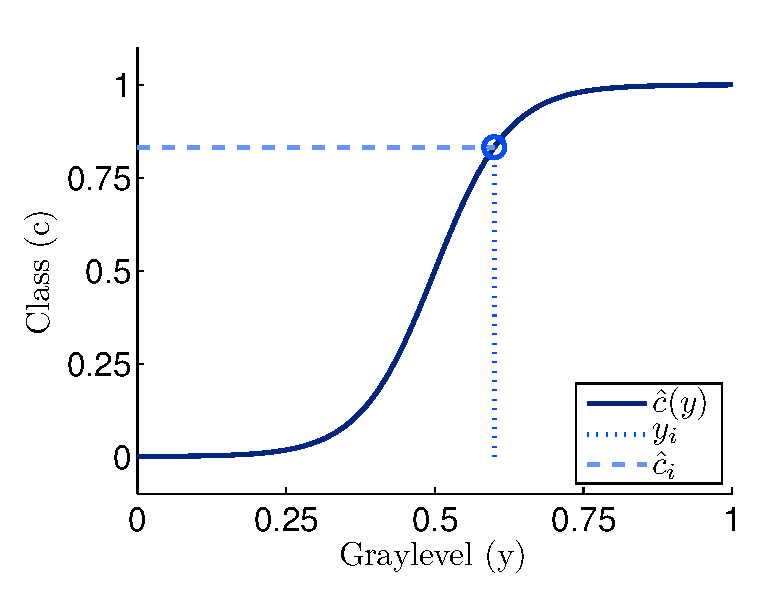
\includegraphics[width=\plotwidth]{lr-basic}
  \caption{The logistic regression model.}
  \label{fig:lr-basic}
\end{figure}
\par
Previous works have not included spatial dimensions in the logistic feature set $\by$, since $\hat{c}$ is not expected to be monotonically related to any spatial dimension.
The circumvention proposed by \citeauthor{Schmidt2015} is to parameterize the feature weights themselves spatially -- that is $\bb\rightarrow\bb(x)$,
\begin{equation}
  \hat{C}(x) = \frac{1}{1+e^{-\eta(x)}},\qquad\eta = \bb(x)^T\bm{Y}(x).
  \label{eq:eq:vlrmodel}
\end{equation}
In this way, the characteristics of the logistic regression model are maintained with respect to graylevel features, but spatial features can have more complex relationships with the output.
A second pre-processing step, however, is now required: standardization of spatial dimensions -- i.e. registration of the input image to a consistent target -- so that the same voxel in every input image corresponds to the same brain region (cf. \S\ \ref{ss:meth-bias+reg} for more details).
Training the VLR model then yields a unique vector $\bb$ for each voxel, or equivalently, one complete image for each parameter.
Such ``parameter images'', as they will be called, are then readily interpretable and can be regularized intuitively.
%Regarding notation in the following subsections: 1) the $(x)$ is omitted here, for clarity, and 2) while only the FLAIR graylevels are used in this implementation, the $\by$ notation is maintained below for compatibility with arbitrary input feature images.
%This approach is similar to the work by \citeauthor{Harmouche2015} \cite{Harmouche2015}, wherein different mixture models are fitted for each of 6 different anatomical regions.
%Since no group statistics are needed in the current model, anatomical parcellations can be replaced by a smooth spatial parametrization.
%The assumptions of this model include the following:
%\begin{itemize}[itemsep=0pt]
%  \item only 2 tissues classes are modelled: WMH and healthy brain tissue;
%  \item image graylevel(s) and spatial location are sufficient features to discriminate the two classes;
%  \item in each voxel, the WMH class is monotonically separable from the healthy class by graylevel(s)
%\end{itemize}
% ==================================================================================================
\subsection{Model Fitting}\label{ss:modelfitting}
Fitting the VLR model involves estimating $\bb$ for each voxel $x$.
This requires some training data: feature vectors from a population of $N$ observations $\bY(x) = \{\bY_1(x),\dots,\bY_{\sn}(x)\}$, and the corresponding labels $\C(x) = \{C_1(x),\dots,C_{\sn}(x)\}$.
Typically, parameter estimation involves maximizing the likelihood of the model, given this data -- i.e. maximum likelihood estimation (MLE).
\par
Three major challenges emerge during model fitting.
These challenges involve contradictions between prior knowledge and the fitted model using the available training data.
That is, these challenges could all be overcome by a more complete training set, but this is rarely available.
The three challenges are:
\begin{enumerate}
  \item \label{chmle:separable} \textbf{Separable classes:} 
  When data from two classes are perfectly separable, the MLE-fitted logistic model can approach a step-function -- i.e. $\b^k\rightarrow+\infty$.
This implies that on either side of a specific graylevel threshold, the model is either 100\% confident in predicting the healthy class, or 100\% confident in predicting the lesion class.
In fact, no threshold is ever so perfect, and instead a level of uncertainty should be maintained around the decision boundary.
These two cases are illustrated in Figure \ref{fig:chmle-sep}.
  \item \label{chmle:sparse} \textbf{Sparsely observed lesion class:} 
  Since WML are often distributed in consistent locations, many brain regions contain no lesions across the entire training dataset.
These voxels will be termed ``healthy training'' voxels, and denoted $\x_{h}$.
In some locations, this is expected (e.g. the GM, since by definition WMH manifest in the WM), while in others, prior knowledge predicts lesions will eventually be observed (e.g. the rest of the WM).
As illustrated in Figure \ref{fig:chmle-noles}, the MLE-fitted model may not maintain the ability to predict $\hat{c} = 1$ in such locations, regardless of the features.
However, the ability to predict lesion should be maintained in many of these locations.
  \item \label{chmle:noisy} \textbf{Smooth parameter images:} 
  It is assumed that similar locations will contain similar training data, yielding smooth parameter images.
If this assumption is sometimes invalid, parameter images could contain noise or discontinuities, creating artifacts in estimated lesion class images.
\end{enumerate}
\begin{figure}
  \centering
  \begin{subfigure}{\plotwidth}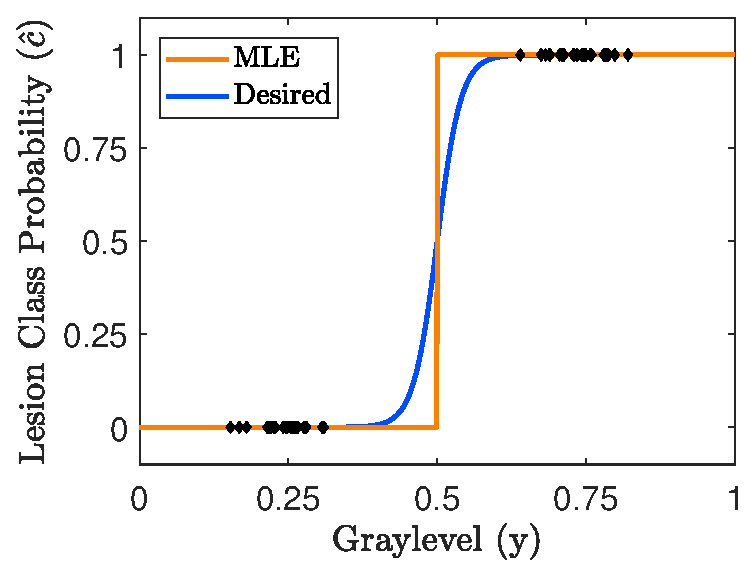
\includegraphics[width=\textwidth]{chmle-sep}  \caption{Separable classes}\label{fig:chmle-sep}  \end{subfigure}
  \begin{subfigure}{\plotwidth}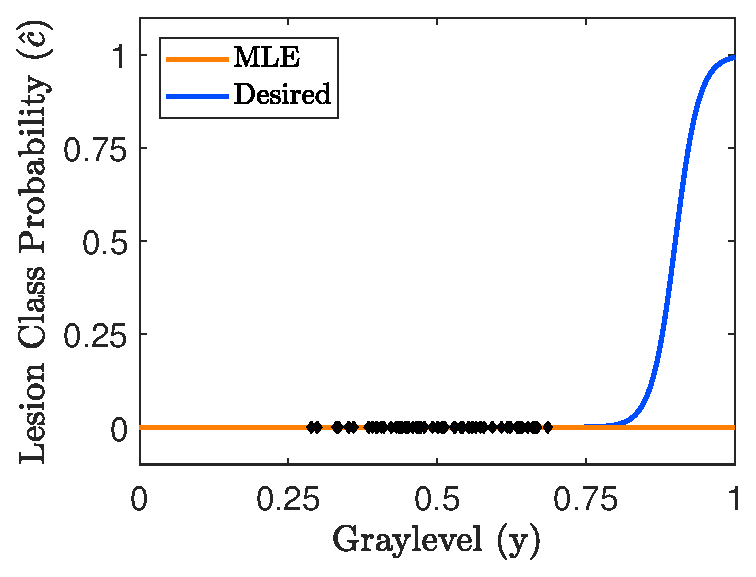
\includegraphics[width=\textwidth]{chmle-noles}\caption{No lesions}       \label{fig:chmle-noles}\end{subfigure}
  \caption{Challenges encountered during estimation of a logistic model.}
  \label{fig:chmle}
\end{figure}
% --------------------------------------------------------------------------------------------------
\subsubsection{Joint Estimation}
In the LPA algorithm, the logistic feature weights for each voxel are not considered independent.
The FLAIR graylevel effect is tied across all voxels -- i.e. $\b^1(x) \rightarrow \b^1$, so $\eta(x) = \b^0(x) + \b^1Y(x)$ -- and a Gaussian MRF model is used to estimate the spatially varying intercept $\b^0(x)$.
This design addresses the aforementioned challenges by greatly increasing the number of observations used to estimate each parameter.
However, it requires joint estimation of all parameters simultaneously, and dramatically increases the complexity of estimation \cite{Schmidt2017a}.
\par
Efficient fitting of such models was the subject of major works by \citeauthor{Schmidt2017} \cite{Schmidt2017,Schmidt2017a}, but several drawbacks remain.
First, Markov Chain Monte Carlo estimation of the model appears to create discontinuity artifacts in the spatial effect image $\b^0(x)$, as shown in Figure \ref{fig:B-lpa}.
Second, MRF modelling of the parameter images assumes that the missing data (i.e. WMH training examples in the more superficial brain regions) can be interpolated spatially, but this may not be justified.
Third, the proposed joint estimation procedures are computationally expensive (versus the methods proposed here), requiring approximately two hours to estimate $\bb(x)$ \cite{Schmidt2017a}.
Finally, it is not clear whether any tied $\b$ are necessary or advantageous in this context.
These deficiencies then motivate investigations into alternative solutions to the above challenges.
\par
In addition to these potential modelling weaknesses, there were also several limitations to the validation methodology for the LPA algorithm, worth noting here.
First, the ``ground truth'' segmentations were generated using an automated algorithm -- the Lesion Growth Algorithm (LGA) \cite{Schmidt2012} of the same toolbox -- rather than a human expert.
Second, the graylevel standardization procedure employed does not consider the variance of image graylevels (only the mean is subtracted); this strongly assumes that user images will have graylevels spanning a similar range.
Third, all 53 training cases were obtained on the same MRI scanner, which may limit generalization performance.
Finally, no segmentation performance results are given in either of the associated publications \cite{Schmidt2017,Schmidt2017a}.
Therefore, while the open-source release of the LPA algorithm is greatly appreciated, significant improvements can be made to this algorithm.
% --------------------------------------------------------------------------------------------------
\subsubsection{Independent Estimation}
An alternative approach is to consider each parameter vector $\bb(x)$ independent.
Doing so greatly simplifies model fitting, but does not address the challenges described above.
These must instead be addressed using regularization strategies, as discussed below in \S\ \ref{s:reg-method}.
In this section, ML estimation of independent parameter vectors $\bb$ is developed.
For clarity, only a single voxel is considered -- i.e. $y$ from $Y(x)$, etc.
\par
As note above, the optimal $\bb$ for each independent voxel can be resolved using MLE.
If the training data are also assumed to be independently observed, then the likelihood (conditioned on the data) is defined from binomial theory as
\begin{align}
  L(\bb\mid\C,\bY) &= \prod_{n=1}^{N} P(c=1\mid\by_n,\bb)^{c_n} \left(1-P(c=1\mid\by_n,\bb)^{1-c_n}\right)\nonumber\\
  &= \prod_{n=1}^{N} \Big[\hat{c}_n^{\en c_n} \left(1-\hat{c}_n^{\en 1-c_n}\right)\Big].
  \label{eq:likelihood}
\end{align}
For computational reasons, it is simpler and asymptotically equivalent to maximize the log-likelihood,
\begin{align}
\L(\bb) &= \log{ \prod_{n=1}^{N} \Big[\hat{c}_n^{\en c_n} \left(1-\hat{c}_n^{\en 1-c_n}\right)\Big] }\nonumber\\
&= \sum_{n=1}^{N} \Big[ c_n \log \hat{c}_n + (1-c_n) \log (1-\hat{c}_n) \Big] \nonumber\\
&= \sum_{n=1}^{N} \Big[ c_n \bb^T\by_n - \log (1+e^{\bb^T\by_n}) \Big].
\label{eq:loglikelihood}
\end{align}
The optimal $\bb$ is therefore resolved by maximizing the log-likelihood,
\begin{align}
\bb^* &= \underset{\bb}{\arg\max} \en\L(\bb)\nonumber\\
&= \underset{\bb}{\arg\max}\en\sum_{n=1}^{N} \Big[ c_n \bb^T\by_n - \log (1+e^{\et\bb^T\by_n}) \Big]
\label{eq:argmaxmle}
\end{align}
% --------------------------------------------------------------------------------------------------
\subsubsection{Iterative Updates}
Estimation of $\bb^*$ can be performed using iterative optimization, using an initial estimate $\bb^{(0)}$ and an update term $\Delta\bb^{(t)}$,
\begin{equation}
\bb^{(t+1)} \leftarrow \bb^{(t)} + \alpha\thinspace\Delta\bb^{(t)},
\label{eq:update}
\end{equation}
where $\alpha$ is a small valued learning rate parameter.
There are many possible definitions of $\Delta\bb$, including simply the gradient of $\L(\bb)$, denoted $\nabla_{\bb}\L$.
However, it can be shown that $\L(\bb)$ is convex, so higher order update equations can be used.
The work by \citeauthor{Minka2003} \cite{Minka2003} compares several options, including Newton's method (and variants), conjugate gradient, iterative scaling (and variants), and dual optimization%
\footnote{Matlab code available at \hreftt{https://github.com/tminka/logreg/}}.
For small feature dimensionality ($K$), performance differences among the options were small.
Classic Newton updates gave a good balance between memory requirements and computational order, so they are used.
\par
If the gradient $\nabla_{\bb}\L$ and Hessian matrix $\nabla^2_{\bb}\L$ are defined as
\begin{align}
\nabla_{\bb}\L &= \left[\begin{array}{c}
\frac{\d L}{\d\b^1}\\\vdots\\\frac{\d L}{\d\b^\sk}
\end{array}\right],\label{eq:llgradient0}\\
\nabla^2_{\bb}\L &= \left[\begin{array}{ccc}
\frac{\d^2 L}{\d\b^1\d\b^1}&\cdots&\frac{\d^2 L}{\d\b^1\d\b^\sk}\\
\vdots&\ddots&\vdots\\
\frac{\d^2 L}{\d\b^\sk\d\b^1}&\cdots&\frac{\d^2 L}{\d\b^\sk\d\b^\sk}
\end{array}\right]\label{eq:llhessian0},
\end{align}
then the Newton update is given by
\begin{equation}
\Delta\bb = -{\nabla^2_{\bb}\L}^{-1}\nabla_{\bb}\L.
\label{eq:newtonmle}
\end{equation}
In the current model, the gradient is given by 
\begin{equation}
\nabla_{\bb}\L = \sum_{n=1}^{N} \by_n\left(c_n - \hat{c}_n\right),
\label{eq:llgradient}
\end{equation}
and the Hessian by
\begin{equation}
\nabla^2_{\bb}\L = \sum_{n=1}^{N} \by_n{\by_n}^T \left(c_n - \hat{c}_n\right).
\label{eq:llhessian}
\end{equation}
Substituting (\ref{eq:llgradient}) and (\ref{eq:llhessian}) into (\ref{eq:newtonmle}), the explicit update $\Delta\bb$ for (\ref{eq:update}) is obtained.
At each iteration, $\Delta\bb^{(t)}$ is re-computed, and the process continues until some convergence criterion is satisfied.
% --------------------------------------------------------------------------------------------------
\subsubsection{Simplification}\label{ss:meth-simple}
It is not necessary to complete the above procedure for all voxels in the standardized space.
Instead, only voxels in the expected location of the brain need to be computed; such voxels can be selected using a binary ``brain mask'', denoted $M(x)$.
More details about the brain mask used in this work can be found in \S\ \ref{ss:brainmask}.
Moreover, since the parameters of each voxel are estimated independently, this can also be computed in parallel.
The details of this implementation are presented in \S\ \ref{s:parallelfit}, after incorporation of the regularizations described in the next section.
\par
Finally, the model has so far been derived in general terms, so that any choice of feature set $\by$ can be used.
However, with only one feature -- the FLAIR graylevel -- it is possible to reparameterize the sigmoid argument as
\begin{align}
\bb^T\by &= \b^0 + \b^1 y^1\nonumber\\
&= s(y-\tau) \qquad\begin{cases} s = \b^1\\ \tau = -\frac{\b^0}{\b^1} \end{cases}.
\label{eq:reparameterize}
\end{align}
In this form, the parameters $\tau$ and $s$ emerge as a graylevel threshold and a slope parameter, respectively.
Specifically, when $y = \tau$, the predicted probability of lesion is $\hat{c} = \tfrac{1}{1+e^{0}} = 0.5$, so $\tau$ controls the location of the class discrimination, as shown in Figure \ref{fig:reparam-t}.
Similarly, the $s$ parameter defines the sensitivity of the logistic function to $y$, as shown in Figure \ref{fig:reparam-s}.
By contrast, varying the original parameter $\beta^1$ with $\beta^0$ constant (Figure \ref{fig:reparam-b1}) results in correlation of these characteristics.
These new parameters, and the corresponding images $\mathcal{T}(x)$ and $\mathcal{S}(x)$, are therefore salient descriptors of the predictive model.
\begin{figure}
  \centering
  \begin{subfigure}{\plotwidth}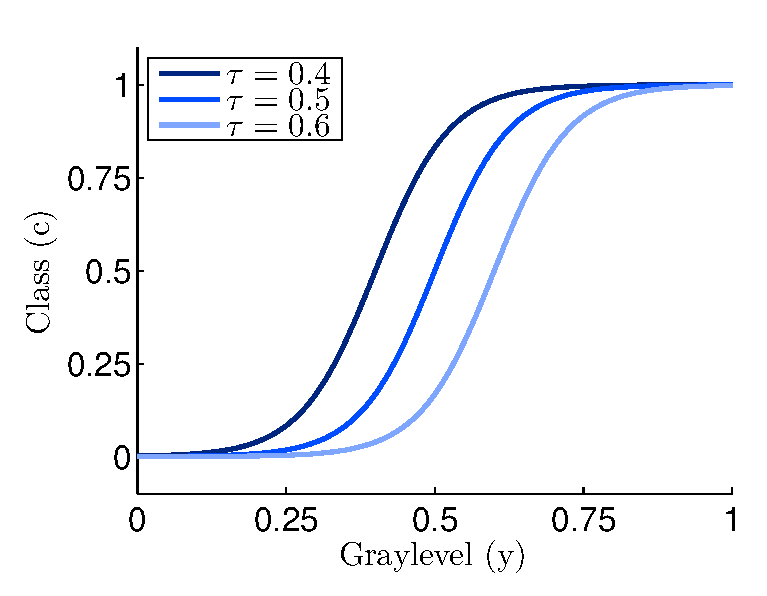
\includegraphics[width=\textwidth]{reparam-t} \caption{Vary $\tau$ with $s = 16$ constant.}\label{fig:reparam-t}\end{subfigure}
  \begin{subfigure}{\plotwidth}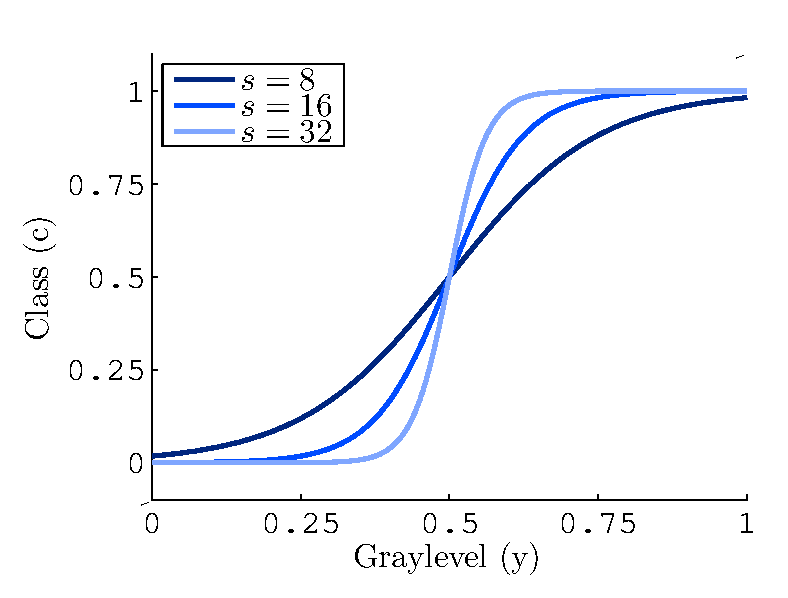
\includegraphics[width=\textwidth]{reparam-s} \caption{Vary $s$ with $\tau = 0.5$ constant.}\label{fig:reparam-s}\end{subfigure}
  \begin{subfigure}{\plotwidth}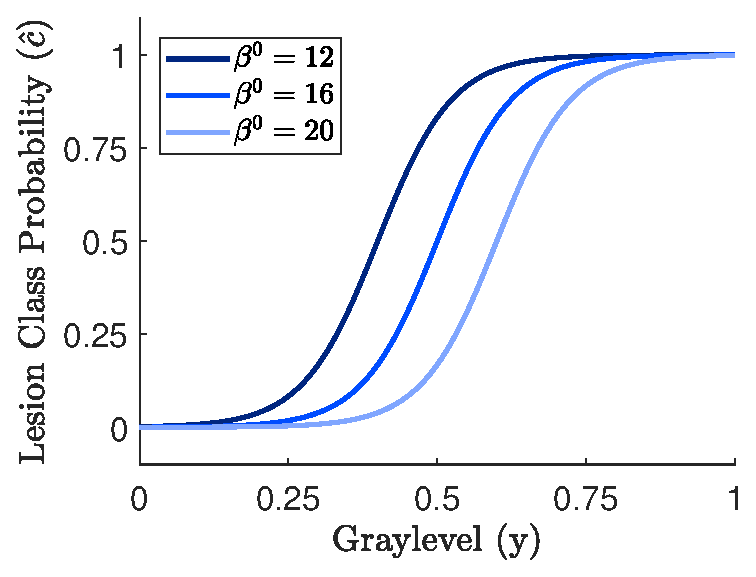
\includegraphics[width=\textwidth]{reparam-b0}\caption{Vary $\b^0$ with $\b^1 = 16$ constant.}\label{fig:reparam-b0}\end{subfigure}
  \begin{subfigure}{\plotwidth}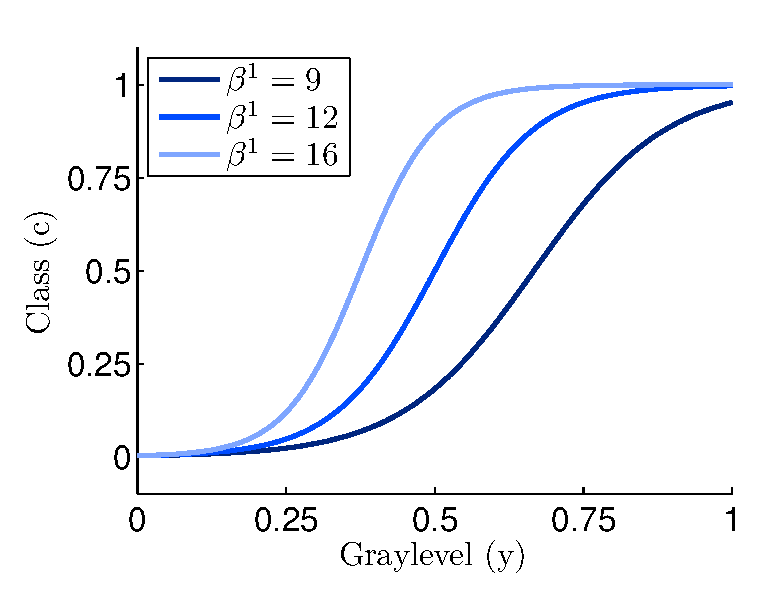
\includegraphics[width=\textwidth]{reparam-b1}\caption{Vary $\b^1$ with $\b^0 = -6$ constant.}\label{fig:reparam-b1}\end{subfigure}
  \caption{Effect of varying the logistic model parameters.}
  \label{fig:reparam}
\end{figure}
%%%%%%%%%%%%%%%%%%%%%%%%%%%%%%%%%%%%%%%%%%%%%%%%%%%%%%%%%%%%%%%%%%%%%%%%%%%%%%%%%%%%%%%%%%%%%%%%%%%%
\section{Regularization}\label{s:method-reg}
Regularizations are methods of injecting prior knowledge about the expected model into the optimization.
Assuming voxel-wise independence of model parameters requires the use of regularization strategies to solve the challenges outlined in \S\ \ref{ss:modelfitting}.
Several regularization methods are explored below.
% ==================================================================================================
\subsection{Data Augmentation}\label{ss:meth-aug}
Noting the central role of training data in each of the challenges, methods of artificially increasing the training dataset size may be particularly useful in solving them.
Data augmentation has long been used in machine learning tasks with limited training data, and there are several methods of generating synthetic data.
In low dimensional input/output spaces, random sampling of fitted class-conditional posterior distributions can produce reasonable samples with known labels \cite{Tanner1987}.
In higher dimensional problem spaces, however, imputation is more difficult \cite{Goodfellow2014}.
For example, the space of potential $100\times100\times100$-sized images has $100^3$ dimensions (one per voxel), yet only a small subspace represents plausible images.
Generating synthetic examples in this space is therefore challenging, especially for segmentation tasks, where the outputs have dimensionality roughly equal to the input.
\par
Alternatively, simple image manipulations can still afford model improvements \cite{Krizhevsky2012}.
In segmentation tasks, both the input image(s) and the corresponding label images can be translated, reflected, rotated, and perhaps resized, thereby avoiding the generation of genuinely synthetic examples.
In the current work, reflections and small (one-voxel) translations can be applied to the label and FLAIR images following registration to the MNI brainspace.
The potential benefits of this augmentation are explored in \S\ \ref{}.
%__JK__ need to define this reference
% ==================================================================================================
\subsection{Classic Regularization}\label{ss:meth-lambda}
The separable classes challenge is well-known in regression problems, and a good solution is to penalize the magnitude of model parameters using the $L_p$-norm: $\lambda\norm{\bb}_p$ \cite{Zou2005}.
It can be shown that $L_1$ regularization corresponds to a Laplacian prior on elements of $\bb$, with scale parameter inversely proportional to $\lambda$ (equivalently, this assumes that the model error follows this distribution).
Similarly, $L_2$ regularization implies a Gaussian prior, with standard deviation inversely proportional to $\lambda$ \cite{Zou2005}.
Model fitting which includes this prior-derived term is called maximum a posteriori (MAP) estimation, and the penalty can be appended to the objective function (\ref{eq:argmaxmle}), as in
\begin{align}
\bb^* &= \underset{\bb}{\arg\max}\en\J(\bb) \nonumber\\
&=\underset{\bb}{\arg\max}\en\L(\bb) - \lambda\norm{\bb}_p \nonumber\\
&= \underset{\bb}{\arg\max}\en\sum_{n=1}^{N} \Big[ c_n \bb^T\by_n - \log (1+e^{\et\bb^T\by_n}) \Big] - \lambda\norm{\bb}_p
\label{eq:argmaxmap}
\end{align}
Due to its relatively large gradient near zero, $L_1$ regularization is typically used to encourage sparsity in the feature weights (i.e. $\b^k\rightarrow0$) \cite{Tibshirani1996}.
This is not desirable in the current model, since the feature (FLAIR graylevel) is known to be discriminative.
Moreover, the expansion of the $\norm{\bb}_1$ term in the gradient of the objective function is not straightforward, since it is non-differentiable at zero \cite{Tibshirani1996,Lee2006}.
Conversely, $L_2$ regularization is more effective at limiting parameter magnitude -- which is the current aim -- and the first and second order gradients of (\ref{eq:argmaxmap}) derive easily \cite{Minka2003}.
For these reasons, only $L_2$ regularization is considered, yielding the following change to the Newton update expression (\ref{eq:newtonmle}),
\begin{align}
\Delta\bb &= -{\nabla^2_{\bb}\J}^{-1}\nabla_{\bb}\J \nonumber\\
&= -{\left(\nabla^2_{\bb}\L-\lambda I\right)}^{-1}\left(\nabla_{\bb}\L-\lambda\bb\right)
\label{eq:newtonmap}
\end{align}
What remains is to select an appropriate value of $\lambda$.
This is explored experimentally in \S\ \ref{ss:toyreg} using a toy model.
% ==================================================================================================
\subsection{Pseudo-Lesions}\label{ss:meth-pseudo}
The sparsely observed lesion class challenge is less common, since discriminative models are rarely fit in the absence of one class altogether.
This occurs here because all voxels are modelled independently.
It is therefore tempting to simply sample features from the lesion class at other spatial locations in order to fit the logistic model in the healthy training voxels, similar to the approach by \citeauthor{Schmidt2017a}.
However, as noted in \S\ \ref{ss:autochallenges} and \S\ \ref{s:modelconcept}, WML are thought to have different intensities in different brain regions \cite{Sled2004,Stevenson2000}, and some locations will likely never contain any WMH.
Considering these facts, the use of deterministic synthetic lesion-class samples, or ``pseudo-lesions'', could instead permit better use of prior knowledge about WMH.
These synthetic observations could be appended to the training data for each voxel so as to minimally balance the training classes, and act as a prior on the distribution of lesion-class features.
%This approach would not be subject to variations in the training data, and it would be feasible to consider the prior probability of healthy tissues (GM / WM / CSF) in the definition.
\par
If the same number of synthetic observations are appended to the training data for each voxel, this is equivalent to appending a number of synthetic images to the training set.
The synthetic feature data are denoted
$\bV(x) = \{\bm{\gamma}_{1}(x),\dots,\bm{\gamma}_{\sv}(x)\}$.
It is assumed that the labels of all synthetic data are ``lesion'', so the set of synthetic label images is simply denoted $\bm{1}(x)$.
The updated training set is therefore $\bY_{\gamma}(x) = \{\bY(x),\bV(x)\}$, and $\bC_{\gamma}(x) = \{\bC(x),\bm{1}(x)\}$.
\par
Design of the synthetic image set $\bV(x)$ should be guided by prior knowledge.
For the same reasons as described above, it is not possible to derive this knowledge from the training set.
Unfortunately, few other sources of structured information are available.
One reasonable approach could make use of healthy tissue prior probability images (Figure \ref{fig:tpm-3}), denoted $\rho(x)$.
Specifically, the expected intensity for the lesion class in each tissue can be multiplied by the tissue probability image, and the results summed to give the overall synthetic image,
\begin{equation}
\gamma(x) = \gamma_{\gm}\cdot\rho_{\gm}(x) + \gamma_{\wm}\cdot\rho_{\wm}(x) + \gamma_{\csf}\cdot\rho_{\csf}(x)
\end{equation}
While WMH are not possible in either the GM or the CSF, it is necessary to select a FLAIR graylevel -- perhaps the maximum possible intensity -- to complete this model.
Additionally, such parameters will inevitably play a role for subjects with imperfect registration or outlier anatomy.
The contributions of pseudo-lesions to model fitting are explored experimentally in \S\ \ref{ss:toyreg}.
%__JK__ should TPMs be introduced sooner?
\begin{figure}[h]
  \centering
  \begin{subfigureside}{$\rho_{\gm}(x)$}\raggedleft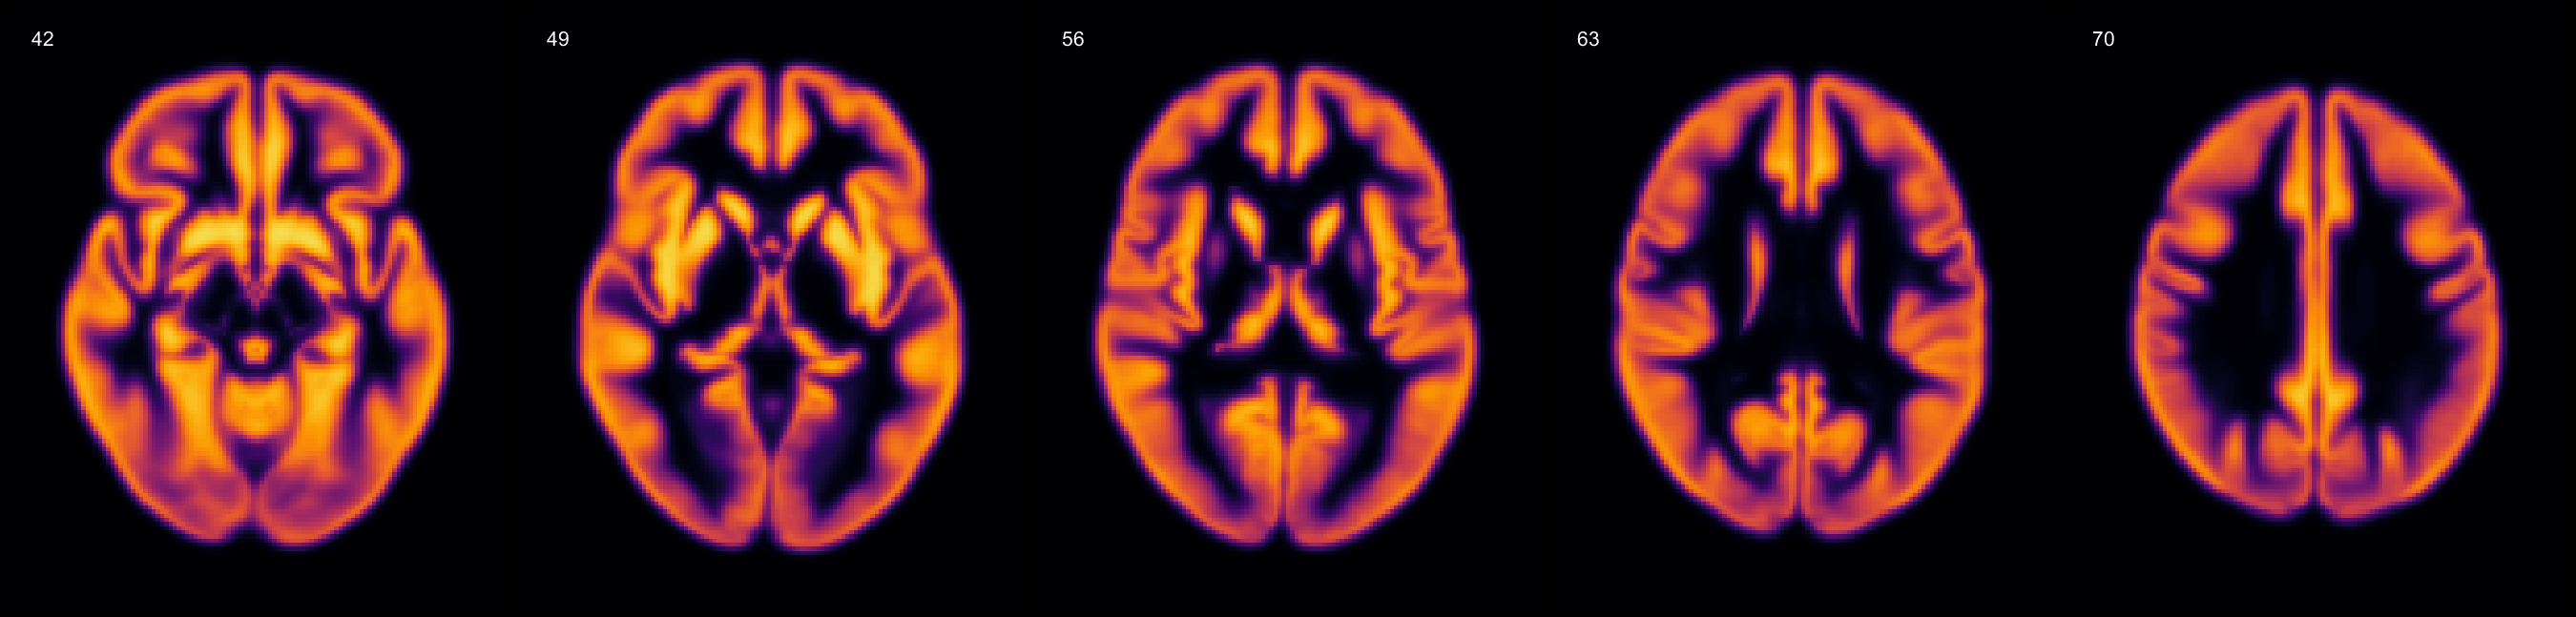
\includegraphics[height=\sliceheight]{tpm-gm.png} 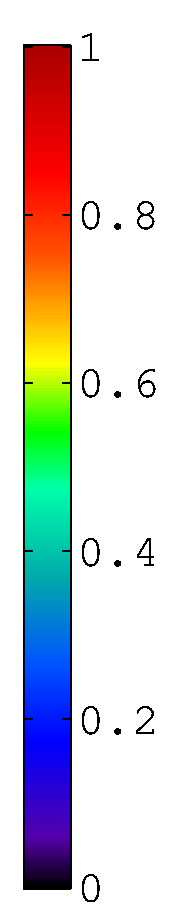
\includegraphics[height=\sliceheight]{cbar-NIH3-0-1}\end{subfigureside}\\[0.5em]
  \begin{subfigureside}{$\rho_{\wm}(x)$}\raggedleft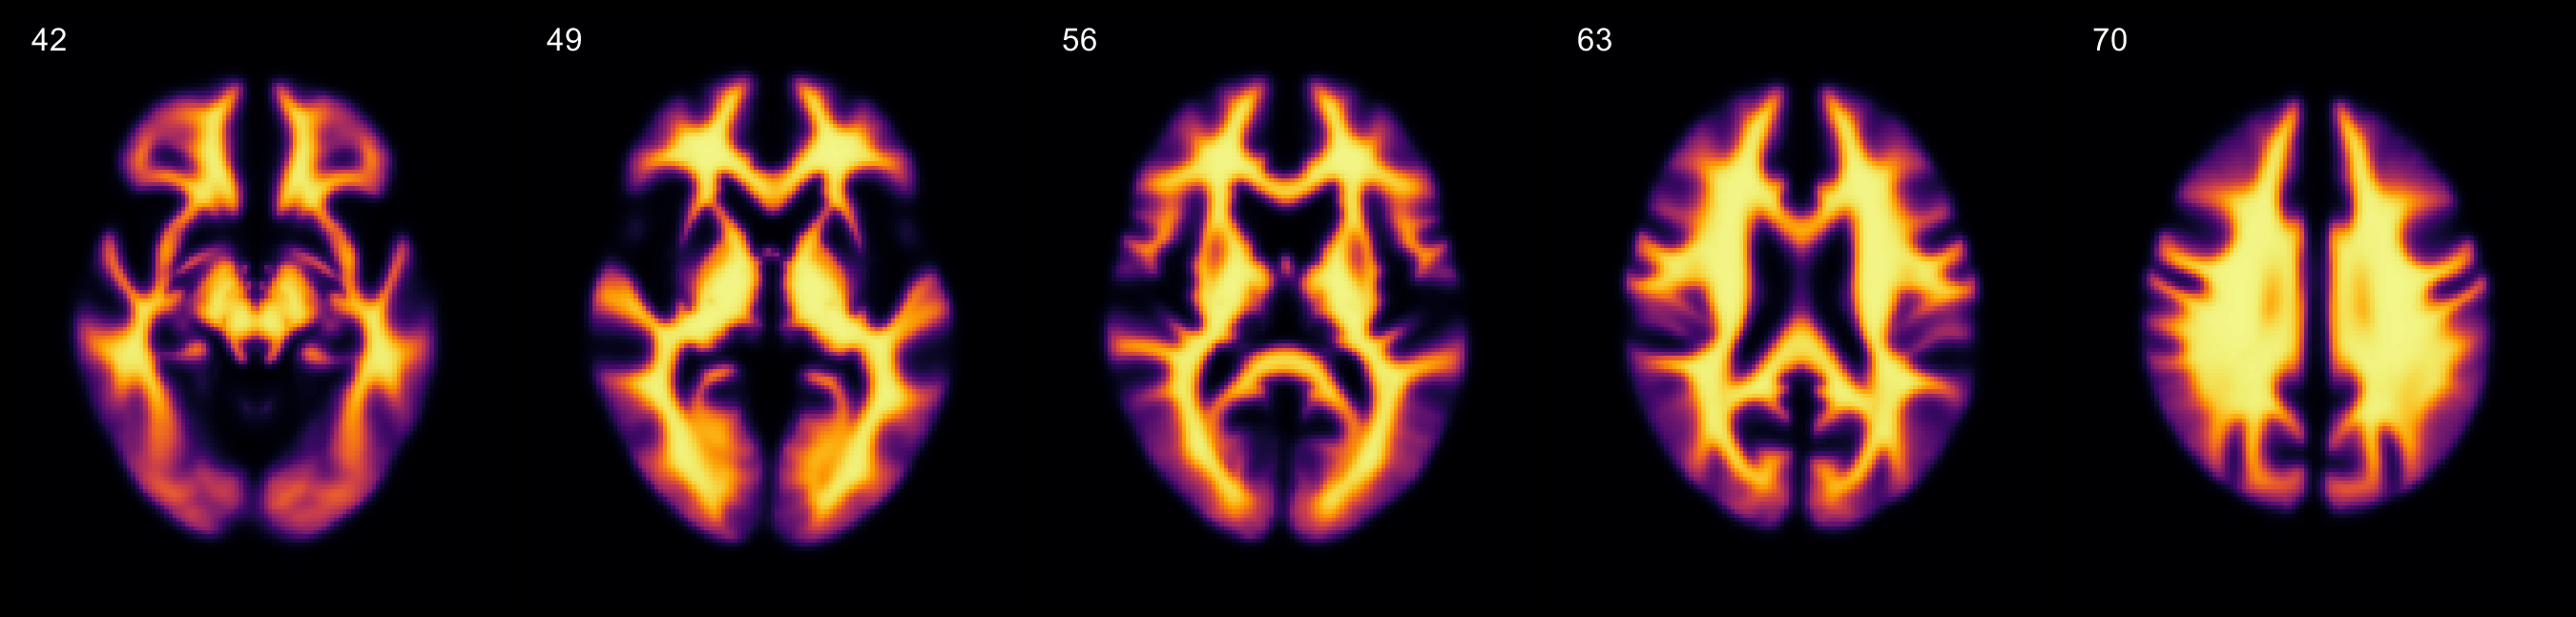
\includegraphics[height=\sliceheight]{tpm-wm.png} 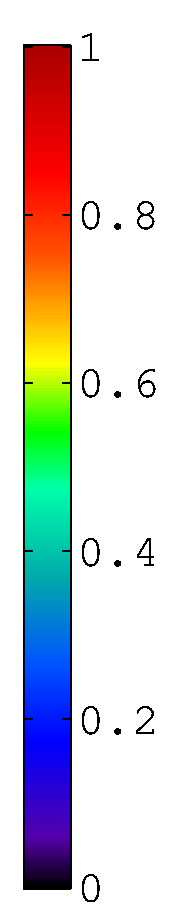
\includegraphics[height=\sliceheight]{cbar-NIH3-0-1}\end{subfigureside}\\[0.5em]
  \begin{subfigureside}{$\rho_{\csf}(x)$}\raggedleft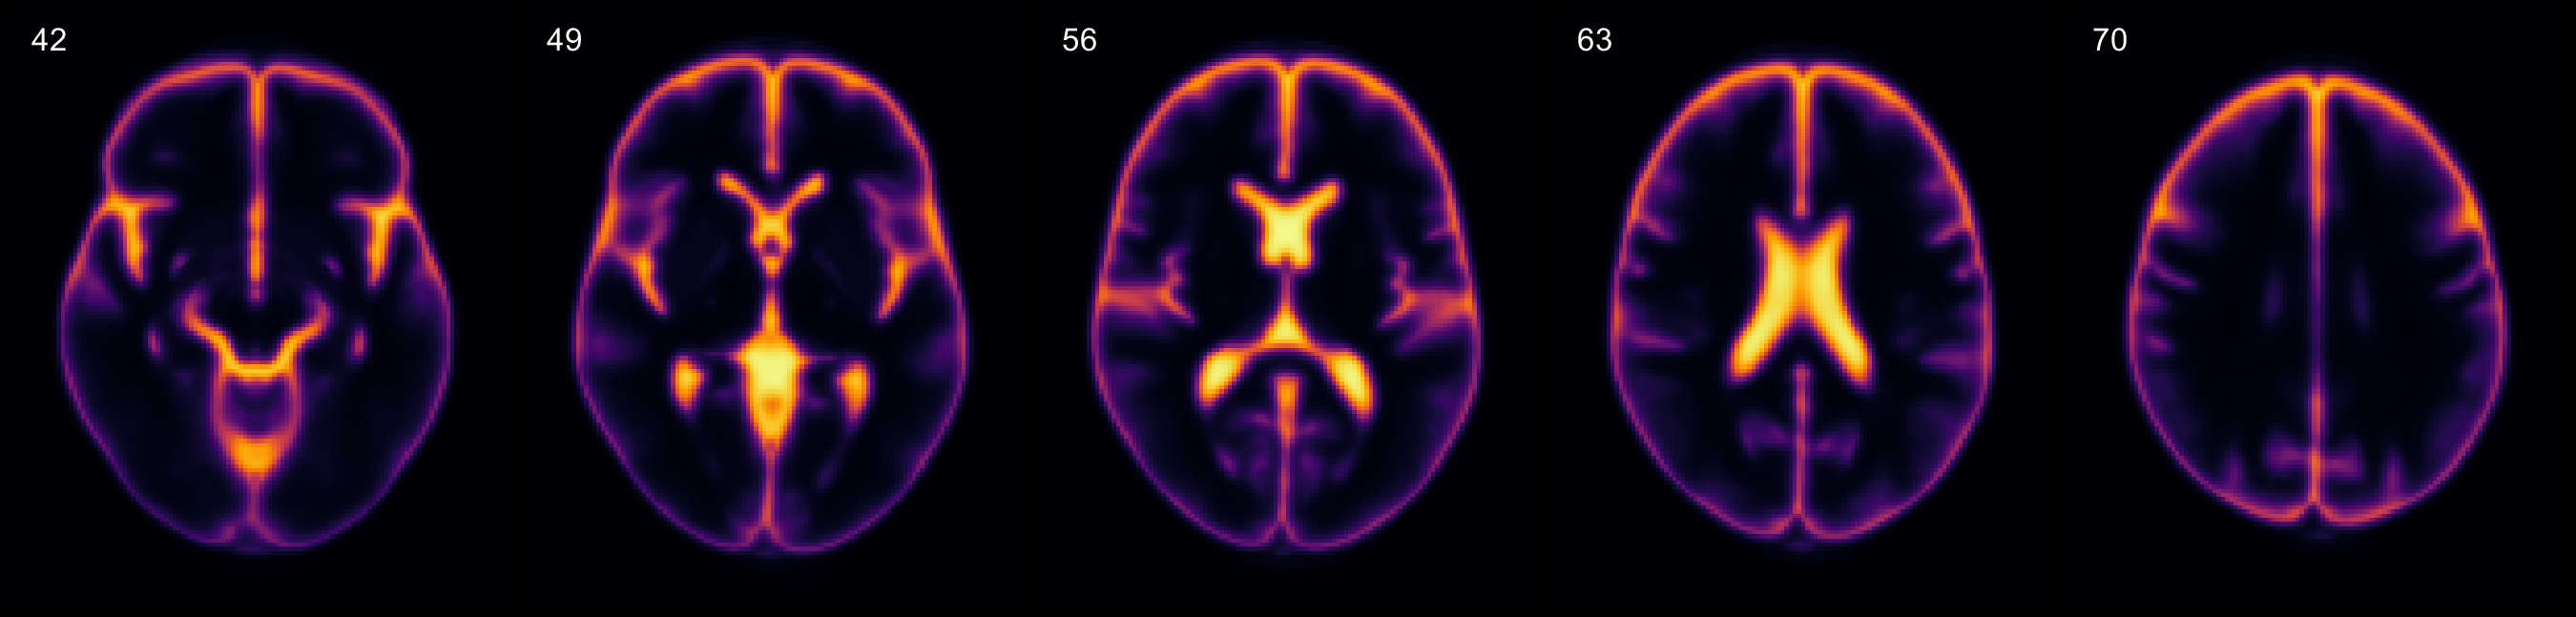
\includegraphics[height=\sliceheight]{tpm-csf.png} 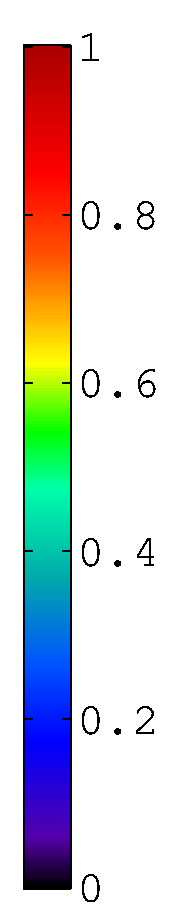
\includegraphics[height=\sliceheight]{cbar-NIH3-0-1}\end{subfigureside}
  \caption{Tissue prior probability images in MNI space. Derived from \cite{Mazziotta2001}.}
  \label{fig:tpm-3}
\end{figure}
% ==================================================================================================
\subsection{Parameter Image Smoothing}\label{ss:meth-smooth}
Finally, independent model fitting in every voxel risks yielding noisy parameter images.
The simplest solution to this problem involves filtering the reconstructed parameter images after estimation.
A wide range of possible filters for this task exist, and a selection of these are summarized in Table \ref{tab:filters}, including the mutable parameters for each.
\begin{table} % __JK__ finish him!
  \centering
  \caption{Image filters considered for smoothing the estimated parameter images.}
  \label{tab:filters}
  \begin{tabular}{llllc}
  	\hline
  	Name                  &   Parameters   & Advantages      & Disadvantages    & Ref. \\ \hline
  	Gaussian              & width $\sigma$ & no artifacts    & blurs edges      &      \\
  	Median                &   width $w$    & preserves edges & square artifacts &      \\
  	Anisotropic Diffusion &                &                 &                  &      \\
  	Bilateral             &                &                 &                  &      \\ \hline
  \end{tabular}
\end{table}
\par
An alternative solution might involve modelling the parameter images as a spatial function (e.g. band-limited discrete cosine / Fourier transform).
However, there are two challenges with this approach.
First, deriving the update gradients for such a model would be challenging, and their computation could significantly increase training time.
Second, such an encoding may introduce artifacts in the resulting parameter images.
Moreover, it is well known that frequency domain band-limiting can be equivalently achieved by convolution (i.e. filtering) in the spatial domain \cite{Gonzalez2006}.
Therefore, only conventional filtering is explored in this work (cf. \S\ \ref{})
%__JK__ define this reference in ch-exp
%__JK__ address MRFs for smoothing here? Check back answer on Quora.
%%%%%%%%%%%%%%%%%%%%%%%%%%%%%%%%%%%%%%%%%%%%%%%%%%%%%%%%%%%%%%%%%%%%%%%%%%%%%%%%%%%%%%%%%%%%%%%%%%%%
\section{Pre-Processing}\label{s:meth-pre}
The proposed VLR classification model addresses several of the challenges outlined in \S\ \ref{ss:autochallenges}.
The problem of overlapping tissue graylevel distributions is mostly solved through expansion of the feature space to include spatial features.
CSF flow-through artifacts, which appear in roughly consistent locations, are similarly managed.
Heterogeneity in the appearance of lesions is also considered by the spatial parametrization of logistic parameters.
Finally, ambiguity regarding moderately hyperintense DAWM, and voxels affected by partial volume effect, is captured in the probabilistic output.
\par
Several challenges, however, still remain.
In particular, a number of assumptions were made about the input data for the VLR model which are likely invalid for raw images.
These assumptions are that:
1) input MRI images are free of bias field artifact;
2) feature intensities are consistent across different subjects;
3) images are consistently sized and voxels represent the same anatomical regions across different subjects.
Solving these challenges must therefore be accomplished by one or more pre-processing steps.
% ==================================================================================================
\subsection{Registration}\label{ss:meth-reg}
Image registration is the process of geometrically transforming a source image so that the image content is aligned per-voxel with a target image of the same subject.
This process facilitates voxel-wise analysis of MRI from different subjects, such as  ``voxel-based morphometry'' \cite{Ashburner2000a} and analysis of functional MRI data \cite{Smith2004}%
\footnote{Incidentally, investigation of these topics were the motivations for developing of the SPM and FSL software packages, respectively.}.
Source images from multiple subjects are usually registered to the same target image; 
in this context, it is useful to define a ``native space'' and a ``standardized space'', denoting the original, subject-specific geometry, and the standardized target geometry.
By convention, the target brain space is usually either the Talairach space \cite{Talairach1988} or the Montreal Neurological Institute (MNI) space \cite{Evans1993}, though any reasonable target image could be used.
\par
Parameters defining registration transforms are fitted by maximizing some measure of overlap between the images \cite{Sotiras2013}.
Simple registration methods employ only affine transformations, comprising a combination of translation, scaling, and shear transformations (e.g. the FLIRT tool \cite{Jenkinson2002} in FSL).
The utility of these methods for neuroimage analysis is limited, since there are often significant differences in brain anatomy between subjects.
Rather, most tools parametrize a spatial warping model, permitting local nonlinear deformations to better match brain structures (e.g.
cubic B-splines in FSL FNIRT \cite{Andersson2007},
discrete cosine transform in SPM Normalize \cite{Ashburner1997,Ashburner2005},
a general diffeomorphism in the SyN algorithm \cite{Avants2008}).
While these models are more difficult to fit, several robust algorithms have been released for general use, with widespread acceptance (e.g. the toolboxes mentioned above).
A \citeyear{Klein2009} comparison of 14 different methods is a good resource on the subject \cite{Klein2009}, while a more recent (\citeyear{Kazemi2014}) study ranks the popular toolboxes SPM, FSL, and Brainsuite \cite{Kazemi2014}.
\par
In the current work, registration is required during both training at testing.
During training, the model parameters $\bb(x)$ are estimated using mutually aligned segmentation examples $\{\bY,\C\}$ in a standard brain space.
At test time (or for actual use), these parameter images are transformed in the opposite direction from the standard space to the native space of the current subject.
Since registration transforms are typically bijections -- i.e. invertible -- the second registration case can be estimated using the same method as the first, minimizing bias.
\par
Unlike other applications, it is not essential that perfect image registration is achieved here.
As noted by \citeauthor{Harmouche2015} \cite{Harmouche2015}, in smoothly varying models, small registration errors can be expected to have a negligible impact.
Therefore, registration was not a primary focus of optimization in this work.
\par
While the registration component of the SPM8 ``Segment'' feature \cite{Ashburner2005} was not among the top performing in the \citeyear{Klein2009} study \cite{Klein2009}, subsequent implementation revisions in SPM12%
\footnote{\hreftt{http://www.fil.ion.ucl.ac.uk/spm/software/spm12/SPM12_Release_Notes.pdf}}
called ``New Segment'' have apparently improved results.
In the \citeyear{Kazemi2014} study \cite{Kazemi2014}, the SPM12 New Segment method achieved the highest Similarity Index of all methods on real (IBSR \cite{IBSR}) data.
\par
Furthermore, the SPM module has several other features amenable to this work.
First, unlike many other registration algorithms, the objective function does not require source and target images to have the same contrast.
This is helpful, since no suitable FLAIR template image is available for use as a target.%
\footnote{One FLAIR template is available in \cite{Winkler2012}; however, this was generated using SPM5, so using it would compound any registration biases associated with the older method.}
Second, it is simple to invoke the SPM modules via the command line or Matlab scripts;
this facilitates smooth integration of this tool in the pipeline.
Third, it is possible to save previously estimated registration transformations, and apply them in the forward or reverse directions efficiently.
This can save significant time during cross validation, since the estimated parameter images $\bm{\b}(x)$ must eventually be transformed to the native space of every subject.
Finally, the SPM ``New Segment'' model additionally estimates the bias field during execution with high accuracy, saving an additional step (cf. \S\ \ref{ss:meth-bias}, below). 
For all these reasons, the registration performed by SPM New Segment was used throughout this work.
After satisfactory visual inspection of all training set images, no other registration tools were investigated.
% ==================================================================================================
\subsection{Bias Correction}\label{ss:meth-bias}
As noted in \S\ \ref{ss:autochallenges}, bias field (\textsc{aka} intensity inhomogeneity), is a smoothly varying intensity variation artifact common in MRI.
The sources of bias field artifact include inhomogeneities in the magnetic field and RF coils used for pulse transmission and signal sensing, as well as non-ideal magnetic properties of the imaged object \cite{Vovk2007}.
The field and coil related sources are more significant at clinical field strengths.
These can be corrected prospectively, though techniques for doing so are limited, and often a small bias field continues to corrupt acquired images \cite{Vovk2007}.
Therefore, retrospective correction has been the subject of much research.
% could use another couple references here...
\par
Similar to image registration, several widely accepted algorithms for estimating and correcting bias field have emerged.
The N3 algorithm \cite{Sled1998}, subsequently updated to N4(ITK) \cite{Tustison2010} and integrated in the FreeSurfer toolbox%
\footnote{\hreftt{https://surfer.nmr.mgh.harvard.edu/}}
is perhaps the most popular, it makes minimal assumptions about the image.
This method aims to sharpen the image histogram by dividing the image by an estimated bias field, parameterized by B-splines for smoothness.
As noted above, the SPM Segment model \cite{Ashburner2005} includes integrated bias field estimation and correction.
The bias field model in this work is parameterized by the discrete cosine transform, as described in in a previous work by \citeauthor{Ashburner2005} \cite{Ashburner1999}.
The FSL Segment feature also estimates bias field in a similar overall model to SPM Segment, except the tissue prior probability maps in SPM are replaced with a Hidden Markov Random Field Model, as described in \cite{Zhang2001}.
Again, two reviews with quantitative performance comparisons provide a good reference of other proposed algorithms, including a comprehensive review in \citeyear{Belaroussi2006} \cite{Belaroussi2006} and a comparison of mainly popular methods in \citeyear{Ganzetti2016} \cite{Ganzetti2016}.
\par
In the \citeyear{Ganzetti2016} comparison \cite{Ganzetti2016}, the authors note that the SPM and FSL models -- which include segmentation -- outperformed the N3 algorithm \cite{Sled1998} and another non-segmenting method \cite{Dawant1993}.
These results are consistent with the advantages of unified generative models described in \S\ \ref{s:modelconcept} and discussed in \citetitle{Ashburner2005} \cite{Ashburner2005}.
Specifically, the estimation of both bias field and tissue segmentation could each be improved if the other was already known.
Rolling these tasks into a single EM-fitted model allows alternating conditional estimates to converge on better results overall.
\par
Bias field estimation was not a primary focus of this work.
Therefore, due to the better performance over N3/4, and the advantages already afforded by SPM Segment for registration noted above, this model was employed for bias correction throughout this work.
No other bias field correction tools were investigated.
% ==================================================================================================
\subsection{Graylevel Standardization}\label{ss:meth-ystd}
The flexibility of image contrast in MRI is a double-edged sword.
This feature, in addition to properties of spatial encoding during acquisition, preclude direct interpretation of image graylevels as a tissue property.
As a result, the same brain region in the same subject may be assigned a different graylevel depending on the MRI sequence time constants, scanner, and spatial acquisition protocol.
For automated analysis of MRI images, therefore, standardization of image graylevels is required.
\par
Graylevel standardization can be achieved using a univariate transformation $\uptau:y\mapsto\tilde{y}$, defined as
\begin{equation}
\tilde{y} = \uptau(y),
\end{equation}
where $\uptau$ is monotonic, and considers characteristics of the input image, such as basic graylevel statistics or the histogram.
The histogram of an image represents the number of occurrences of each graylevel in the image.
Normalizing the histogram by the total number of voxels $X$ yields the the probability mass function (PMF) $f_{\sy}(y)$,
\begin{align}
f_{\sy}(y) &= \frac{1}{X}h_{\sy}(y)\nonumber\\
&= \frac{1}{X}\sum_{i=1}^{X}
\begin{cases}
1&Y(x_i) = y\\
0&Y(x_i) \ne y\\
\end{cases}
\end{align}
The cumulative density function (CDF) $F_{\sy}(y)$ is the cumulative sum of $f_{\sy}(y)$,
\begin{equation}
F_{\sy}(y) = \sum_{\gamma=y_{\min}}^{y} f_{\sy}(\gamma)
\end{equation}
The PMF of an MRI can be decomposed into the contributions of each constituent tissue, as shown in Figure \ref{fig:simflairplot}.
This is the fundamental principle underlying mixture models (cf. \S\ \ref{ss:priorproposed}).
The goal of standardization is therefore to align these sub-distributions as closely as possible.
\par
Previously proposed methods of standardizing MRI intensities include the following:%
\footnote{This section considers only univariate standardization methods, since only FLAIR intensities are used in this work.}
\begin{itemize}
  \item \textbf{Range Matching:}
  The simplest approach to standardization involves rescaling the data using the minimum and maximum intensities,
  \begin{equation}\uptau(y) = \frac{y-y_{\min}}{y_{\max}-y_{\min}}.\end{equation}
  Naively, this method is very susceptible to corruption by outliers.
  For more robustness, $y_{\min}$ and $y_{\max}$ can be defined using intensity quantiles -- e.g. $[\epsilon_1,1-\epsilon_2]$.
  However, selection of an appropriate $\epsilon_2$ for WMH segmentation is difficult, since WMH typically constitute only the top 1\% of the total brain volume.
  Furthermore, differences in image contrasts are not considered by this approach.
  \item \textbf{Statistical standardization:}
  Another simple but popular approach uses the first and second order moments of the PMF,
  \begin{equation}\uptau(y) = \frac{y-\mu_{\sy}}{\sigma_{\sy}}.\end{equation}
  As with range matching, variable image contrasts are not well modelled by this method.
  \item \textbf{Histogram equalization:}
  Histogram equalization transforms the image PMF to a uniform distribution, thereby distributing image intensities equally across the available range.
  The desired transform  is defined as the CDF of the input image (cf. \cite{Gonzalez2006} for derivation),
  \begin{equation}\uptau(y) = F_{\sy}(y).\end{equation}
  The chief assumption of histogram equalization for standardization is that input images contain consistent amounts of each tissue class.
  In MRI with WMH, this assumption may not be valid; however, this technique may still have value.
  \item \textbf{Histogram matching:}
  Histogram matching is similar to histogram equalization, except that the output PMF is not uniform, but some other specified distribution, $f_{\tilde{\sy}}$.
  This transform is defined as the function composition of the input CDF and the inverse target CDF,
  \begin{equation}\uptau(y) = {F_{\tilde{\sy}}}^{-1}\big(F_{\sy}(y)\big)\end{equation}
  Histogram matching 
  (cf. \ref{ss:hm-vs-he} for an illustration and experimental evidence.)
  \item \textbf{Nyul standardization:}
  In \cite{Nyul1999,Nyul2000}, \citeauthor{Nyul1999} proposed a method for intensity standardization which has subsequently been used in other works.
  This method defines $\uptau$ with piecewise linear segments connecting the $Q$ quantiles of the input PMF $q$, with quantiles of a target PMF $r$,
  \begin{equation}\uptau(y) = r_i + \left(y-q_i\right)\left(\frac{r_{i+1}-r_i}{q_{i+1}-q_i}\right),\quad y\in[q_i,q_{i+1}]\end{equation}
  However, it can be shown that this transformation is a non-uniform trapezoidal Riemann approximation of true histogram matching, which performs worse in terms of intensity standardization.%
  \footnote{This result is presented and supported with experiments in \cite{Knight2017}.}
  \item \textbf{Regional characteristics}
  Decorrelating variation in intensities from variability in anatomical content is a central challenge in intensity standardization.
  One solution is to define the image-specific transformation using characteristics from a more anatomically consistent brain region.
  This is the approach employed by \citeauthor{Shinohara2014} in the so-called white stripe method \cite{Shinohara2014}.
  In the current work, this region, denoted $\x_{\uptau}$, can be defined in MNI space using tissue priors (Figure \ref{fig:tpm-3}), anatomical label maps, or any other method of selecting a subset of voxels.
\end{itemize}
% --------------------------------------------------------------------------------------------------
\subsubsection{Quantifying Standardization}
While the major advantages and challenges to several graylevel standardization methods have been briefly noted, it remains to explore the utility of each experimentally.
In the current work, the goal of this step is to maximize the separation of the two classes.
This can even be maximized voxel-wise, due to the characteristics of the VLR model.
Therefore, an intermediate objective function $\Z$ should be defined which quantifies the degree of separation of the two classes.%
\footnote{Alternatively, the entire pipeline can be executed under cross validation and overall performance compared between standardization methods.
However this does not consider potential interactions between the standardization method and tunable downstream parameters.}
This objective function can then be used to optimize any tunable parameters in each of the transforms -- e.g. $\bm{\epsilon}$, $Q$, $\x_{\uptau}$ -- and also to select the best overall method.
\par
Two such functions are proposed.
The first is discrete, and inspired by the Zero-Crossing Rate \cite{Kedem1986}.
It measures the number of class transitions in the sorted feature data $\tilde{\Y}_s$, as shown in Figures \ref{fig:jsep-diff-1} and \ref{fig:jsep-diff-2}.
With $\C_s$ as the class labels after sorting by the feature $\tilde{\Y} = \uptau(\Y)$, the objective function $\Z_{\Delta}$ is defined as
\begin{equation}
\Z_{\Delta} = \sum_{n=1}^{N-1}\begin{cases}
1&\C_s^{n} \ne \C_s^{n+1}\\
0&\C_s^{n}  =  \C_s^{n+1}
\end{cases}.
\end{equation}
This function is discrete and bounded, as in $\Z_{\Delta}\in\mathbb{Z}\left[1,\lfloor\frac{N}{2}\rfloor\right]$%
\footnote{The lower bound can be zero if one class is not observed.}
and the lower bound is optimal -- i.e. $\Z_{\Delta}$ should be minimized.
\par
The second function is continuous, and inspired by probability theory.
It measures the relative overlap of class distributions, $p(\tilde{y}\mid c=1)$ and $p(\tilde{y}\mid c=0)$, estimated using kernel smoothing, as shown in Figures \ref{fig:jsep-conv-1} and \ref{fig:jsep-conv-2}.
This objective function $\Z_{\star}$ can be defined as
\begin{equation}
\Z_{\star} = \int_{\tilde{y}_{\min}}^{\tilde{y}_{\max}}
\frac{\min\{p(\gamma \mid c=1), p(\gamma \mid c=0)\}}
     {\max\{p(\gamma \mid c=1), p(\gamma \mid c=0)\}}\d\gamma,
\qquad p(\gamma \mid c) \approx \sum_{\tilde{y}\in\{\tilde{\Y}\mid c\}}\delta(\gamma-\tilde{y}) \star G_{\sigma}(\gamma)
\end{equation}
where $G_{\sigma}(\gamma)$ is a Gaussian convolution kernel with width $\sigma$.
This function is continuous and bounded, as in $\Z_{\Delta}\in\left[0,1\right]$, and the lower bound is again optimal.
\par
\begin{figure}
  \centering
  \begin{subfigure}{\plotwidth}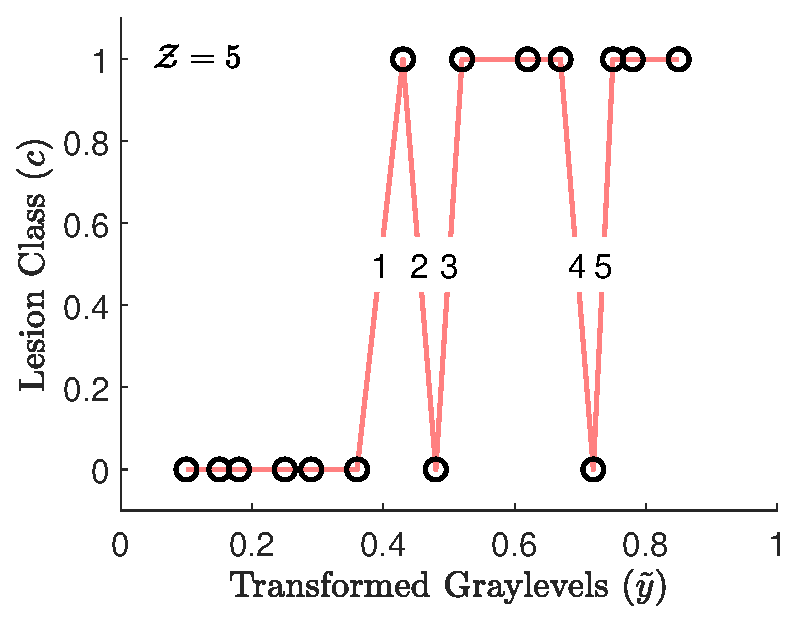
\includegraphics[width=\textwidth]{jsep-diff-1}\caption{$\Z_{\Delta}$ with overlapping classes}\label{fig:jsep-diff-1}\end{subfigure}
  \begin{subfigure}{\plotwidth}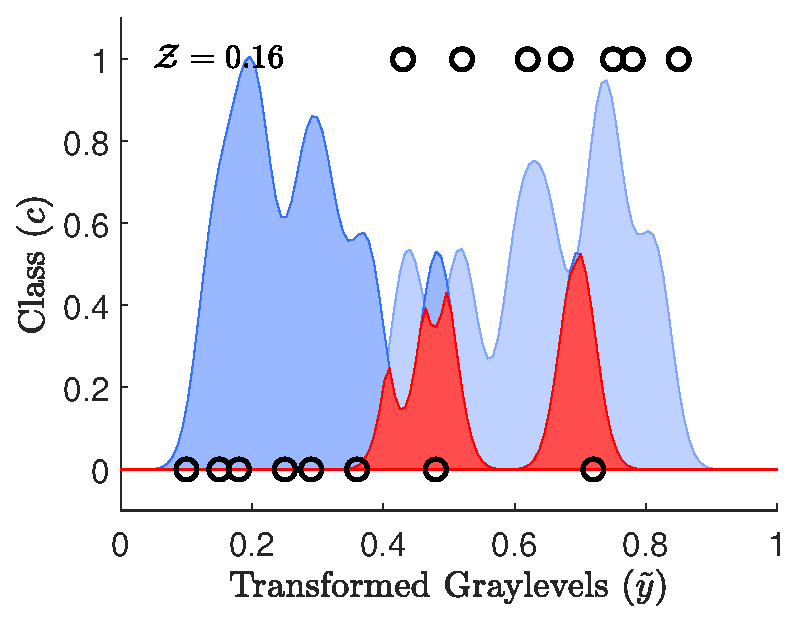
\includegraphics[width=\textwidth]{jsep-conv-1}\caption{$\Z_{\star}$ with overlapping classes}\label{fig:jsep-conv-1}\end{subfigure}\\[1em]
  \begin{subfigure}{\plotwidth}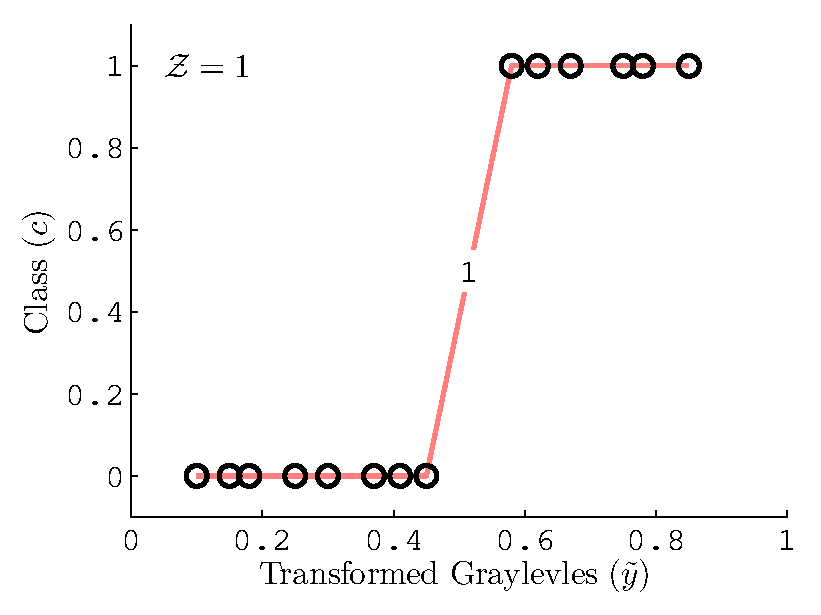
\includegraphics[width=\textwidth]{jsep-diff-2}\caption{$\Z_{\Delta}$ with separable classes}\label{fig:jsep-diff-2}\end{subfigure}
  \begin{subfigure}{\plotwidth}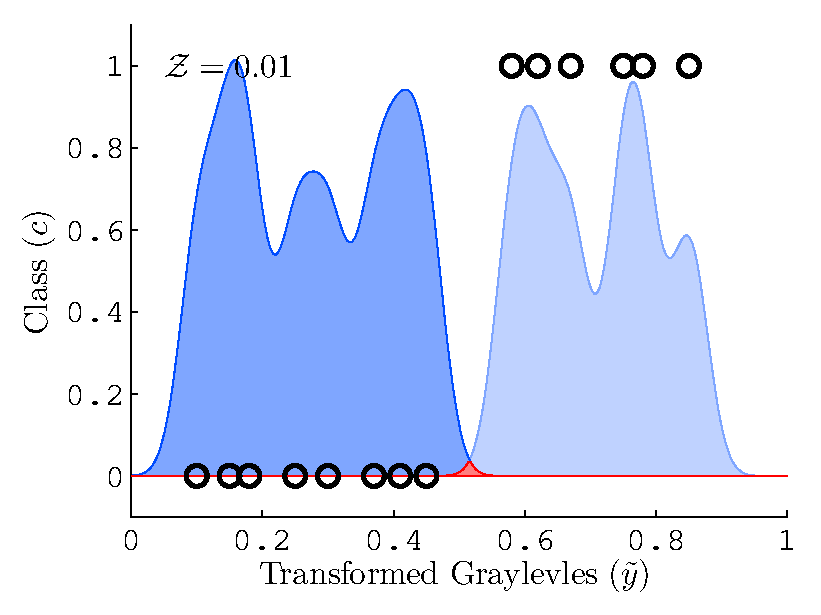
\includegraphics[width=\textwidth]{jsep-conv-2}\caption{$\Z_{\star}$ with separable classes}\label{fig:jsep-conv-2}\end{subfigure}
  \caption{Illustration of potential separability objective functions.}
  \label{fig:jsep}
\end{figure}
% --------------------------------------------------------------------------------------------------
\subsubsection{Supervised Standardization}
At this point, it is not hard to see that it should be possible to estimate an optimal graylevel standardization transform using the training data.
That is, a \textit{supervised graylevel standardization}.%
\footnote{To the best of this author's knowledge, such a technique has never been proposed.}
If $\Z$ is differentiable, then this optimization can be performed using gradient descent, or similar methods.
Unfortunately, neither of the above objective functions $\Z$ were reasonably differentiable, but many other optimization paradigms which do not require gradients could be used.
% some examples? is this genetic algorithms?
%%%%%%%%%%%%%%%%%%%%%%%%%%%%%%%%%%%%%%%%%%%%%%%%%%%%%%%%%%%%%%%%%%%%%%%%%%%%%%%%%%%%%%%%%%%%%%%%%%%%
\section{Post-Processing}\label{s:meth-post}
The 

Following pre-processing and classification by the VLR model, 
  
In principle, post-processing aims to incorporate any additional knowledge of the problem which has not been considered in upstream elements. 




\clearpage
%%%%%%%%%%%%%%%%%%%%%%%%%%%%%%%%%%%%%%%%%%%%%%%%%%%%%%%%%%%%%%%%%%%%%%%%%%%%%%%%%%%%%%%%%%%%%%%%%%%%
\section{Segmentation Performance Metrics}\label{ss:metrics}
Quantifying the performance of a model is essential to optimizing its design.
Typically, WMH segmentation performance is characterized in two respects: voxel-wise agreement and total lesion load (LL) volume agreement.
When comparing the estimated class $\hat{c}$ to the ground truth class $c$, each individual voxel can occupy one of four states (colours shown for future reference):
\begin{itemize}[itemsep=0pt,topsep=0pt]
  \item[\textcolor{green}{\scalebox{0.7}{$\blacksquare$}}] True Positive (TP): $c = 1$ and $\hat{c} = 1$, correctly predicted ``lesion''.
  \item[\textcolor{red}  {\scalebox{0.7}{$\blacksquare$}}] False Positive (FP): $c = 0$ and $\hat{c} = 1$, incorrectly predicted ``lesion''.
  \item[\textcolor{blue} {\scalebox{0.7}{$\blacksquare$}}] False Negative (FN): $c = 1$ and $\hat{c} = 0$, incorrectly predicted ``healthy''.
  \item[\textcolor{black}{\scalebox{0.7}{$\blacksquare$}}] True Negative (TN): $c = 0$ and $\hat{c} = 0$, correctly predicted ``healthy''.
\end{itemize}
Summing the number of voxels in each state over an entire image volume, voxel-wise agreement can then be quantified using the following measures:
\begin{itemize}
  \item \textbf{Similarity Index (SI)}
  (\textsc{aka} Dice Similarity Coefficient, F1-Score)\\
  Measures overall segmentation performance.
  \begin{equation}SI = \dfrac{2TP}{2TP + FP + FN}\end{equation}
  \item \textbf{Precision (Pr)}
  (\textsc{aka} Overlap Fraction, Positive Predictive Value)\\
  Fraction of predicted predicted positives which are true positives.
  \begin{equation}Pr = \dfrac{TP}{TP+FP}\end{equation}
  \item \textbf{Recall (Re)}
  (\textsc{aka} Sensitivity, True Positive Rate)\\
  Fraction of true positives which are predicted positive.
  \begin{equation}Re = \dfrac{TP}{TP+FN}\end{equation}
\end{itemize}
Each measure is $\in [0,1]$, where higher is better.
Note that typical performance metrics like accuracy and sensitivity are avoided, since they include the $TN$ count in the numerator, which is typically much larger than $TP + FP + FN$ combined -- i.e. $c=1$ is a rare event.
\par
Overall volume agreement between segmentations is characterized using the 2-way mixed-effects single-rater absolute intraclass correlation coefficient (ICC)%
\footnote{Option \texttt{`A-1'} in the Matlab function \texttt{ICC} from \hreftt{https://www.mathworks.com/matlabcentral/fileexchange/22099}}\ 
\cite{Koo2016}, while trends in over/undersegmentation with lesion load are illustrated using Blant-Altman plots \cite{Altman1983}.
%%%%%%%%%%%%%%%%%%%%%%%%%%%%%%%%%%%%%%%%%%%%%%%%%%%%%%%%%%%%%%%%%%%%%%%%%%%%%%%%%%%%%%%%%%%%%%%%%%%%
\section{Model Summary}



A summary of the model is shown in Figure \ref{fig:modelsum}.
\begin{figure}
  \centering\scalebox{0.65}{\pgfdeclarelayer{background}
\pgfdeclarelayer{foreground}
\pgfsetlayers{background,main,foreground}
\tikzset{%
  arrow/.style = { ->, >=Latex,  very thick, rounded corners, draw = #1!60!white },
  input/.style = { ->, >=Latex, ultra thick, rounded corners, draw = red },
  clr/.style   = { ultra thick, rounded corners, fill = #1!60!white },
  image/.style = { fill = black, draw = black!80!white, ultra thick, inner sep = 0 },
  plot/.style  = { fill = white, inner sep = 0 },
  label/.style = { fill = white, fill opacity = 0, text opacity = 1 },
  tbox/.style  = { fill = white, draw = #1!60!white, very thick, align = center }
}
\newcommand*{\img}[3]{%
  \node[image] at (#1,#2){\includegraphics[width=\ixx cm, height=\iyy cm]{#3}}; % chktex 1
}
\newcommand*{\imgt}[4]{%
	\img{#1}{#2}{#3}
	\begin{pgfonlayer}{foreground}
		\node[label] at (#1,#2-\iy-0.4){\large #4};
	\end{pgfonlayer}
}
\newcommand*{\plot}[5]{%
  \node[plot] at (#1,#2){\includegraphics[width=#3cm, height=#4cm]{#5}};
}
\newcommand*{\voxpath}[4]{%
  \filldraw[fill=black!20!white,draw=black]
  (#1,#2)--(#1+\vw,#2)--(#1+#3,#2-#3+\vw)--(#1+#3-\vw,#2-#3+\vw)--(#1,#2);
  \filldraw[fill=black!20!white,draw=black]
  (#1,#2)--(#1,#2-\vw)--(#1+#3-\vw,#2-#3)--(#1+#3-\vw,#2-#3+\vw)--(#1,#2);
  \filldraw[fill=black!20!white,draw=black]
  (#1+#3,#2-#3)--(#1+#3,#2-#3+\vw)--(#1+#3-\vw,#2-#3+\vw)--(#1+#3-\vw,#2-#3)--(#1+#3,#2-#3);
  \node[below right] at (#1+#3,#2-#3) {#4};
}
\newcommand*{\imgstack}[5]{%
  \foreach \x in {0,...,#3}{\img{#1-0.1*#3+0.1*\x}{#2+0.1*#3-0.1*\x}{#4}} % chktex 11 chktex 1
  \begin{pgfonlayer}{foreground}
	  \node[label] at (#1,#2-\iy-0.4){\large #5};
	\end{pgfonlayer}{foreground}
}
\newcommand*{\imgvoxstack}[5]{%
	\voxpath{#1+\vw+0.3-0.1*#3-\vl-\vl}
					{#2-\vw-0.2+0.1*#3+\vl+\vl}{\vl}{}
	\imgstack{#1}{#2}{#3}{#4}{#5}
	\voxpath{#1+\vw+0.3}
	        {#2-\vw-0.2}{\vl}{}
}
\newcommand*{\textbox}[6]{%
  \node[tbox=#5,minimum width=#3cm,minimum height=#4cm]at(#1,#2){#6};
}
%\newcommand*{\blocktitle}[4]{%
%  \node[title=#3]at(#1,#2){#4};
%  \fill[clr=#3](#1+0.6,#2+1.7)--(#1+0.6,#2-1.7)--(#1+0.6+0.3,#2);
%}
\newcommand*{\vw}{0.1}
\newcommand*{\vl}{0.7}
\newcommand*{\ix}{0.8}\newcommand*{\ixx}{1.6}
\newcommand*{\iy}{1}  \newcommand*{\iyy}{2}
\newcommand*{\pw}{1.5}
\newcommand*{\fw}{0.3}

% --------------------------------------------------------------------------------------------------
\begin{tikzpicture}
    \useasboundingbox(1.5, 0.0) rectangle (24.0, 20.5);
    \begin{pgfonlayer}{background}
      % background boxes
      \draw[black!30!white,rounded corners,very thick](-0.25, 0.25) rectangle (23.75, 9.75);
      \draw[black!30!white,rounded corners,very thick](-0.25,10.25) rectangle (23.75,20.00);
      % box labells
      \node[fill=black!10!white,rounded corners,minimum width=3cm, minimum height=1.0cm]
        at(21.75,19.00){\textsc{Training}};
      \node[fill=black!10!white,rounded corners,minimum width=3cm, minimum height=1.0cm]
        at(21.75, 8.75){\textsc{Testing}};
      %\draw[step=0.5,black!10!white,very thin](-0.5, 0.0) grid (24.0,20.0);
    \end{pgfonlayer}
    % training
    \imgt       { 1.0}{18.0}{c1}{$\mathrm{C}_1(x)$}
    \imgt       { 1.0}{14.0}{c2}{$\mathrm{C}_{\textsc{n}}(x)$}
    \imgt       { 3.0}{18.0}{i1}{$\mathrm{Y}_1(x)$}
    \imgt       { 3.0}{14.0}{i2}{$\mathrm{Y}_{\textsc{n}}(x)$}
    \node[font=\fontsize{30}{0}\selectfont,align=center] at ( 1.0,15.8) {$\vdots$};
    \node[font=\fontsize{30}{0}\selectfont,align=center] at ( 3.0,15.8) {$\vdots$};
    \imgstack   {10.0}{16.0}{6}{ir} {$\mathcal{Y}(x)$}
    \imgvoxstack{13.0}{16.0}{6}{jr} {$\tilde{\mathcal{Y}}(x)$}
    \imgvoxstack{13.0}{12.0}{6}{c1} {$\mathcal{C}(x)$}
    \plot       {17.5}{14.0}{4}{4}  {lr-fit}
    \imgvoxstack{22.0}{14.0}{1}{bb} {$\bm{\beta}(x)$}
    % testing
    \imgstack   { 3.0}{ 2.0}{1}{bb} {$\bm{\beta}(x)$}
    \imgvoxstack{ 3.0}{ 6.0}{0}{it} {$Y_{test}(x)$}
    \imgvoxstack{10.0}{ 2.0}{1}{bb} {$\bm{\upbeta}(x)$}
    \imgvoxstack{10.0}{ 6.0}{0}{jt} {$\tilde{\mathrm{Y}}_{test}(x)$}
    \plot       {14.5}{ 4.0}{4}{4}  {lr-test}
    \imgvoxstack{19.0}{ 4.0}{0}{qt} {$\hat{\mathrm{C}}_{test}(x)$}
    \imgt       {22.0}{ 4.0}{lt}    {$\hat{\mathrm{C}}_{test}^{\circ}(x)$}
    % training arrows
    \draw[arrow={blue}  ]( 3.0+\ix,18.0    )--( 3.5+\ix,18.0)--( 3.5+\ix,16.0)--( 5.0,16.0);
    \draw[arrow={blue}  ]( 3.0+\ix,16.0    )--( 5.0    ,16.0);
    \draw[arrow={blue}  ]( 3.0+\ix,14.0    )--( 3.5+\ix,14.0)--( 3.5+\ix,16.0)--( 5.0,16.0);
    \draw[arrow={blue}  ]( 8.0    ,16.0    )--(10.0-\ix,16.0);
    \draw[arrow={blue}  ]( 1.0    ,12.3    )--( 1.0    ,12.0)--( 5.0,    12.0);
    \draw[arrow={blue}  ]( 5.0    ,12.0    )--(13.0-\ix,12.0);
    \draw[arrow={blue},dotted](6.5,16.0    )--( 6.5    ,12.5);
    \draw[arrow={violet}](10.0    ,16.0+\iy)--(10.0    ,18.5);
    \draw[arrow={violet}](11.5,    19.0    )--(13.0    ,19.0)--(13.0,16.0+\iy);
    \draw[arrow={red}   ](13.0+\ix,16.0    )--(14.5    ,16.0)--(14.5,14.0)--(15.5,14.0);
    \draw[arrow={red}   ](13.0+\ix,12.0    )--(14.5    ,12.0)--(14.5,14.0)--(15.5,14.0);
    \draw[arrow={red}   ](19.5    ,14.0    )--(22.0-\ix,14.0);
    % testing arrows
    \draw[arrow={blue}  ]( 3.0+\ix, 6.0    )--( 5.0    , 6.0);
    \draw[arrow={blue},dotted](6.5, 6.0    )--( 6.5    , 2.5);
    \draw[arrow={blue}  ]( 3.0+\ix, 2.0    )--( 5.0    , 2.0);
    \draw[arrow={blue}  ]( 8.0    , 2.0    )--(10.0-\ix, 2.0);
    \draw[arrow={violet}]( 6.5    , 6.5    )--( 6.5    , 8.0);
    \draw[arrow={violet}]( 8.0    , 8.5    )--(10.0    , 8.5)--(10.0    , 6.0+\iy);
    \draw[arrow={red}   ](10.0+\ix, 6.0    )--(11.5    , 6.0)--(11.5, 4.0)--(12.5, 4.0);
    \draw[arrow={red}   ](10.0+\ix, 2.0    )--(11.5    , 2.0)--(11.5, 4.0)--(12.5, 4.0);
    \draw[arrow={red}   ](16.5    , 4.0    )--(19.0-\ix, 4.0);
    \draw[arrow={orange}](19.0    , 4.0+\iy)--(19.0    , 6.5);
    \draw[arrow={orange}](20.5,     7.0    )--(22.0    , 7.0)--(22.0, 4.0+\iy);
    % training texts
    \textbox    { 6.5}{16.0}{3}{1.0}{blue}  {Bias Correction\\\& Registration}
    \textbox    { 6.5}{12.0}{3}{1.0}{blue}  {Same Transform\\Applied}
    \textbox    {10.0}{19.0}{3}{1.0}{violet}{Histogram\\Matching}
    \textbox    {17.5}{17.0}{4}{1.0}{red}   {Logistic Regression\\Model Fitting}
    % testing texts
    \textbox    { 6.5}{6.25}{3}{0.5}{blue}  {Bias Correction}
    \textbox    { 6.5}{5.75}{3}{0.5}{blue}  {Registration}
    \textbox    { 6.5}{ 2.0}{3}{1.0}{blue}  {Inverse Transform\\Applied}
    \textbox    { 6.5}{ 8.5}{3}{1.0}{violet}{Histogram\\Matching}
    \textbox    {14.5}{ 7.0}{4}{1.0}{red}   {Logistic Regression\\Lesion Prediction}
    \textbox    {19.0}{ 7.0}{3}{1.0}{orange}{Post\\Processing}
\end{tikzpicture}}
  \caption{Overview of the proposed algorithm.
    Typefaces -- upright Roman: images in native space; italic Roman: images in standard (MNI) space; calligraphic: a set of images from several patients; bold: a set of images corresponding to different features;
    Variables -- $C(x)$: manual segmentation; $Y(x)$: FLAIR image, $\beta(x)$: parameter image; $\hat{C}(x)$: estimated lesion segmentation.}
  \label{fig:modelsum}
\end{figure}
% ==================================================================================================
\subsection{Tunable Parameters}
In order to achieve the best possible model performance, it is prudent to track tunable model parameters (\textsc{aka} hyperparameters) which are distinct from those fitted during each cross validation fold.
Considering both the main VLR model and the pre- and post-processing aspects, the parameters of the proposed algorithm are summarized in Table \ref{tab:hyperparams} and also programmatically in \nameref{m:hypdef.m}.
The optimization of these model components will be the subject of the next chapter.
\begin{table}
  \centering
  \caption{Model hyperparameters.}
  \label{tab:hyperparams}
  \begin{tabular}{lllll}
  	\hline
  	Stage                            & Parameter            & Notation                    & Type                                              & Default                   \\ \hline
  	\multirow{4}{*}{Pre-Processing}  & Reflect Augmentation & $A_R$                       & $\mathbb{B}$                                      & $0$                       \\
  	                                 & Shift Augmentation   & $A_S$                       & $\mathbf{N}_p$                                    & $\mathbf{N}_0$            \\
  	                                 & Graylevel Transform  & $T_y$                       & $f: y\mapsto \tilde{y}$                           & $f_{he}$                  \\
  	                                 & Transform Mask       & $M_{T}(x)$                  & $\mathbb{B}(x)$                                   & $M_{\text{brain}}$        \\ \hline
  	\multirow{6}{*}{VLR Fitting}     & Iterations           & $N_{t}^{\lr}$               & $\mathbb{Z}$                                      & $30$                      \\
  	                                 & Initial $\bb$        & $\bb^{(0)}$                 & $\Re^2$                                           & $[0,0]$                   \\
  	                                 & Learning Rate        & $\alpha$                    & $\Re$                                             & $1$                       \\
  	                                 & Regularization       & $\lambda$                   & $\Re$                                             & $0$                       \\
  	                                 & Pseudo-Lesions       & $\{\bY_{\rho},\bC_{\rho}\}$ & $\{\{\et\cdot\in\Re\},\{\et\cdot\in[0,1]\}\}$     & $\{\{\},\{\}\}$           \\
  	                                 & $\bb$ Filter         & $F_{\bb}$                   & $f: \bb(\mathbf{N}_p(x)) \mapsto \tilde{\bb}(x)$  & $\tilde{\bb}(x) = \bb(x)$ \\ \hline
  	\multirow{3}{*}{Post-Processing} & Min Lesion  Size     & $\mathrm{x}_{\min}^{c}$     & $\Re\en(\text{mm}^{3})$                           & $0$                       \\
  	                                 & MRF Iterations       & $N_{t}^{\mrf}$              & $\mathbb{Z}$                                      & $0$                       \\
  	                                 & MRF Weights          & $W_{\mrf}$                  & $\{w_{\Delta},w_{F},w_y\}$                        & $\{1,1,1\}$               \\ \hline
  \end{tabular}
  \tablepost{Notation. $\mathbb{B}$: boolean value; $\mathbb{Z}$: integer value; $\mathbb{R}^n$: real value ($n=1$) or vector ($n > 1$); $\mathbf{N}_p$: nearest $p$ voxel neighbourhood.}
\end{table}
% --------------------------------------------------------------------------------------------------
% ==================================================================================================
%%%%%%%%%%%%%%%%%%%%%%%%%%%%%%%%%%%%%%%%%%%%%%%%%%%%%%%%%%%%%%%%%%%%%%%%%%%%%%%%%%%%%%%%%%%%%%%%%%%%
